%  A simple AAU report template.
%  2015-05-08 v. 1.2.0
%  Copyright 2010-2015 by Jesper Kjær Nielsen <jkn@es.aau.dk>
%
%  This is free software: you can redistribute it and/or modify
%  it under the terms of the GNU General Public License as published by
%  the Free Software Foundation, either version 3 of the License, or
%  (at your option) any later version.
%
%  This is distributed in the hope that it will be useful,
%  but WITHOUT ANY WARRANTY; without even the implied warranty of
%  MERCHANTABILITY or FITNESS FOR A PARTICULAR PURPOSE.  See the
%  GNU General Public License for more details.
%
%  You can find the GNU General Public License at <http://www.gnu.org/licenses/>.
%
%  A simple AAU report template.
%  2015-05-08 v. 1.2.0
%  Copyright 2010-2015 by Jesper Kjær Nielsen <jkn@es.aau.dk>
%
%  This is free software: you can redistribute it and/or modify
%  it under the terms of the GNU General Public License as published by
%  the Free Software Foundation, either version 3 of the License, or
%  (at your option) any later version.
%
%  This is distributed in the hope that it will be useful,
%  but WITHOUT ANY WARRANTY; without even the implied warranty of
%  MERCHANTABILITY or FITNESS FOR A PARTICULAR PURPOSE.  See the
%  GNU General Public License for more details.
%
%  You can find the GNU General Public License at <http://www.gnu.org/licenses/>.
%
\documentclass[11pt,twoside,a4paper,openright]{report}
%%%%%%%%%%%%%%%%%%%%%%%%%%%%%%%%%%%%%%%%%%%%%%%%
% Language, Encoding and Fonts
% http://en.wikibooks.org/wiki/LaTeX/Internationalization
%%%%%%%%%%%%%%%%%%%%%%%%%%%%%%%%%%%%%%%%%%%%%%%%
% Select encoding of your inputs. Depends on
% your operating system and its default input
% encoding. Typically, you should use
%   Linux  : utf8 (most modern Linux distributions)
%            latin1 
%   Windows: ansinew
%            latin1 (works in most cases)
%   Mac    : applemac
% Notice that you can manually change the input
% encoding of your files by selecting "save as"
% an select the desired input encoding. 
\usepackage[utf8]{inputenc}
% Make latex understand and use the typographic
% rules of the language used in the document.
\usepackage[danish,english]{babel}
% Use the palatino font
\usepackage[sc]{mathpazo}
\linespread{1.05}         % Palatino needs more leading (space between lines)
% Choose the font encoding
\usepackage[T1]{fontenc}
%%%%%%%%%%%%%%%%%%%%%%%%%%%%%%%%%%%%%%%%%%%%%%%%
% Graphics and Tables
% http://en.wikibooks.org/wiki/LaTeX/Importing_Graphics
% http://en.wikibooks.org/wiki/LaTeX/Tables
% http://en.wikibooks.org/wiki/LaTeX/Colors
%%%%%%%%%%%%%%%%%%%%%%%%%%%%%%%%%%%%%%%%%%%%%%%%
% load a colour package
\usepackage{xcolor}
\definecolor{aaublue}{RGB}{33,26,82}% dark blue
% The standard graphics inclusion package
\usepackage{graphicx}
% Set up how figure and table captions are displayed
\usepackage{caption}
\captionsetup{%
  font=footnotesize,% set font size to footnotesize
  labelfont=bf % bold label (e.g., Figure 3.2) font
}
% Make the standard latex tables look so much better
\usepackage{array,booktabs}
% Enable the use of frames around, e.g., theorems
% The framed package is used in the example environment
\usepackage{framed}

%%%%%%%%%%%%%%%%%%%%%%%%%%%%%%%%%%%%%%%%%%%%%%%%
% Mathematics
% http://en.wikibooks.org/wiki/LaTeX/Mathematics
%%%%%%%%%%%%%%%%%%%%%%%%%%%%%%%%%%%%%%%%%%%%%%%%
% Defines new environments such as equation,
% align and split 
\usepackage{amsmath}
% Adds new math symbols
\usepackage{amssymb}
% Use theorems in your document
% The ntheorem package is also used for the example environment
% When using thmmarks, amsmath must be an option as well. Otherwise \eqref doesn't work anymore.
\usepackage[framed,amsmath,thmmarks]{ntheorem}

%%%%%%%%%%%%%%%%%%%%%%%%%%%%%%%%%%%%%%%%%%%%%%%%
% Page Layout
% http://en.wikibooks.org/wiki/LaTeX/Page_Layout
%%%%%%%%%%%%%%%%%%%%%%%%%%%%%%%%%%%%%%%%%%%%%%%%
% Change margins, papersize, etc of the document
\usepackage[
  inner=28mm,% left margin on an odd page
  outer=41mm,% right margin on an odd page
  %top=,
  %bottom=,
  ]{geometry}
% Modify how \chapter, \section, etc. look
% The titlesec package is very configureable
\usepackage{titlesec}
\titleformat{\chapter}[display]{\normalfont\huge\bfseries}{\chaptertitlename\ \thechapter}{20pt}{\Huge}
\titleformat*{\section}{\normalfont\Large\bfseries}
\titleformat*{\subsection}{\normalfont\large\bfseries}
\titleformat*{\subsubsection}{\normalfont\normalsize\bfseries}
%\titleformat*{\paragraph}{\normalfont\normalsize\bfseries}
%\titleformat*{\subparagraph}{\normalfont\normalsize\bfseries}

% Clear empty pages between chapters
\let\origdoublepage\cleardoublepage
\newcommand{\clearemptydoublepage}{%
  \clearpage
  {\pagestyle{empty}\origdoublepage}%
}
\let\cleardoublepage\clearemptydoublepage

% Change the headers and footers
\usepackage{fancyhdr}
\pagestyle{fancy}
\fancyhf{} %delete everything
\renewcommand{\headrulewidth}{0pt} %remove the horizontal line in the header
\fancyhead[RE]{\small\nouppercase\leftmark} %even page - chapter title
\fancyhead[LO]{\small\nouppercase\rightmark} %uneven page - section title
\fancyhead[LE,RO]{\thepage} %page number on all pages, header
% \fancyfoot[LE,RO]{Page \thepage\space of \pageref{LastPage}} %page number on all pages, footer
% Do not stretch the content of a page. Instead,
% insert white space at the bottom of the page
\raggedbottom
% Enable arithmetics with length. Useful when
% typesetting the layout.
\usepackage{calc}

%%%%%%%%%%%%%%%%%%%%%%%%%%%%%%%%%%%%%%%%%%%%%%%%
% Bibliography
% http://en.wikibooks.org/wiki/LaTeX/Bibliography_Management
%%%%%%%%%%%%%%%%%%%%%%%%%%%%%%%%%%%%%%%%%%%%%%%%
%\usepackage[backend=biber,
%  bibencoding=utf8,
%  style=numeric,
%  sorting = none,
%  %citestyle=apa,
%  language=danish,
%  ]{biblatex}
%\usepackage{url}


\usepackage[square]{natbib}

\bibliographystyle{unsrtnat} % viser referencers url

\usepackage[hyphens]{url} % url formatering
\usepackage{hyperref}

%\usepackage{babel/polyglossia}
\usepackage{csquotes}

%%%%%%%%%%%%%%%%%%%%%%%%%%%%%%%%%%%%%%%%%%%%%%%%
% Misc
%%%%%%%%%%%%%%%%%%%%%%%%%%%%%%%%%%%%%%%%%%%%%%%%
% Add bibliography and index to the table of
% contents
\usepackage[nottoc]{tocbibind}
% Add the command \pageref{LastPage} which refers to the
% page number of the last page
\usepackage{lastpage}
% Add todo notes in the margin of the document
\usepackage[
%  disable, %turn off todonotes
  colorinlistoftodos, %enable a coloured square in the list of todos
  textwidth=\marginparwidth, %set the width of the todonotes
  textsize=scriptsize, %size of the text in the todonotes
  ]{todonotes}

%%%%%%%%%%%%%%%%%%%%%%%%%%%%%%%%%%%%%%%%%%%%%%%%
% Hyperlinks
% http://en.wikibooks.org/wiki/LaTeX/Hyperlinks
%%%%%%%%%%%%%%%%%%%%%%%%%%%%%%%%%%%%%%%%%%%%%%%%
% Enable hyperlinks and insert info into the pdf
% file. Hypperref should be loaded as one of the 
% last packages
\usepackage{hyperref}
\hypersetup{%
	plainpages=false,%
	pdfauthor={Author(s)},%
	pdftitle={Title},%
	pdfsubject={Subject},%
	bookmarksnumbered=true,%
	colorlinks=false,%
	citecolor=black,%
	filecolor=black,%
	linkcolor=black,% you should probably change this to black before printing
	urlcolor=black,%
	pdfstartview=FitH%
}


% skriv \par for halvt linieskift 
\setlength{\parindent}{0em}    %bestemmer indrykning på linie
\setlength{\parskip}{0.5em}    %bestemmer størrelse af linieskift

\usepackage{float}
\usepackage{booktabs}
\usepackage{enumitem}

\usepackage{amssymb}

\usepackage{longtable}

\usepackage{makecell}

\newlength\mytemplength

\newcommand\parboxc[3]{%
    \settowidth{\mytemplength}{#3}%
    \parbox[#1][#2]{\mytemplength}{\centering #3}%
}


\usepackage{listings}

%Coding:
\usepackage[newfloat]{minted}
\usepackage{caption}
\newenvironment{code}{\captionsetup{type=listing}}{}
\SetupFloatingEnvironment{listing}{name=Code example}

\usepackage{csquotes}

% Viser mere info om fejl
%\setcounter{errorcontextlines}{999}% package inclusion and set up of the document
% see, e.g., http://en.wikibooks.org/wiki/LaTeX/Formatting#Hyphenation
% for more information on word hyphenation
\hyphenation{ex-am-ple hy-phen-a-tion short}
\hyphenation{long la-tex}
% 
%  A simple AAU report template.
%  2015-05-08 v. 1.2.0
%  Copyright 2010-2015 by Jesper Kjær Nielsen <jkn@es.aau.dk>
%
%  This is free software: you can redistribute it and/or modify
%  it under the terms of the GNU General Public License as published by
%  the Free Software Foundation, either version 3 of the License, or
%  (at your option) any later version.
%
%  This is distributed in the hope that it will be useful,
%  but WITHOUT ANY WARRANTY; without even the implied warranty of
%  MERCHANTABILITY or FITNESS FOR A PARTICULAR PURPOSE.  See the
%  GNU General Public License for more details.
%
%  You can find the GNU General Public License at <http://www.gnu.org/licenses/>.
%
%
%
% see, e.g., http://en.wikibooks.org/wiki/LaTeX/Customizing_LaTeX#New_commands
% for more information on how to create macros

\DeclareCaptionType{use_case}[Use Case]
\DeclareCaptionType{actor}[Actor]

%%%%%%%%%%%%%%%%%%%%%%%%%%%%%%%%%%%%%%%%%%%%%%%%
% Macros for the titlepage
%%%%%%%%%%%%%%%%%%%%%%%%%%%%%%%%%%%%%%%%%%%%%%%%
%Creates the aau titlepage
\newcommand{\aautitlepage}[3]{%
  {
    %set up various length
    \ifx\titlepageleftcolumnwidth\undefined
      \newlength{\titlepageleftcolumnwidth}
      \newlength{\titlepagerightcolumnwidth}
    \fi
    \setlength{\titlepageleftcolumnwidth}{0.5\textwidth-\tabcolsep}
    \setlength{\titlepagerightcolumnwidth}{\textwidth-2\tabcolsep-\titlepageleftcolumnwidth}
    %create title page
    \thispagestyle{empty}
    \noindent%
    \begin{tabular}{@{}ll@{}}
      \parbox{\titlepageleftcolumnwidth}{
        \iflanguage{danish}{%
          
\includegraphics[width=\titlepageleftcolumnwidth]{figures/aau_logo_da}
        }{%
          
\includegraphics[width=\titlepageleftcolumnwidth]{figures/aau_logo_en}
        }
      } &
      \parbox{\titlepagerightcolumnwidth}{\raggedleft\sf\small
        #2
      }\bigskip\\
       #1 &
      \parbox[t]{\titlepagerightcolumnwidth}{%
      \textbf{Abstract:}\bigskip\par
        \fbox{\parbox{\titlepagerightcolumnwidth-2\fboxsep-2\fboxrule}{%
          #3
        }}
      }\\
    \end{tabular}
    \vfill
    \iflanguage{danish}{%
      \noindent{\footnotesize\emph{Rapportens indhold er frit tilgængeligt, men offentliggørelse (med kildeangivelse) må kun ske efter aftale med forfatterne.}}
    }{%
      \noindent{\footnotesize\emph{The content of this report is freely available, but publication (with reference) may only be pursued due to agreement with the author.}}
    }
    \clearpage
  }
}

%Create english project info
\newcommand{\englishprojectinfo}[8]{%
  \parbox[t]{\titlepageleftcolumnwidth}{
    \textbf{Title:}\\ #1\bigskip\par
    \textbf{Theme:}\\ #2\bigskip\par
    \textbf{Project Period:}\\ #3\bigskip\par
    \textbf{Project Group:}\\ #4\bigskip\par
    \textbf{Participant(s):}\\ #5\bigskip\par
    \textbf{Supervisor(s):}\\ #6\bigskip\par
    %\textbf{Copies:} #7\bigskip\par
    \textbf{Page Numbers:} \pageref{LastPage}\bigskip\par
    \textbf{Date of Completion:}\\ #8
  }
}

%Create danish project info
\newcommand{\danishprojectinfo}[8]{%
  \parbox[t]{\titlepageleftcolumnwidth}{
    \textbf{Titel:}\\ #1\bigskip\par
    \textbf{Tema:}\\ #2\bigskip\par
    \textbf{Projektperiode:}\\ #3\bigskip\par
    \textbf{Projektgruppe:}\\ #4\bigskip\par
    \textbf{Deltager(e):}\\ #5\bigskip\par
    \textbf{Vejleder(e):}\\ #6\bigskip\par
    \textbf{Oplagstal:} #7\bigskip\par
    \textbf{Sidetal:} \pageref{LastPage}\bigskip\par
    \textbf{Afleveringsdato:}\\ #8
  }
}

%%%%%%%%%%%%%%%%%%%%%%%%%%%%%%%%%%%%%%%%%%%%%%%%
% An example environment
%%%%%%%%%%%%%%%%%%%%%%%%%%%%%%%%%%%%%%%%%%%%%%%%
\theoremheaderfont{\normalfont\bfseries}
\theorembodyfont{\normalfont}
\theoremstyle{break}
\def\theoremframecommand{{\color{gray!50}\vrule width 5pt \hspace{5pt}}}
\newshadedtheorem{exa}{Example}[chapter]
\newenvironment{example}[1]{%
		\begin{exa}[#1]
}{%
		\end{exa}
}
% my new macros

\begin{document}
%frontmatter
\pagestyle{empty} %disable headers and footers
\pagenumbering{roman} %use roman page numbering in the frontmatter
%  A simple AAU report template.
%  2015-05-08 v. 1.2.0
%  Copyright 2010-2015 by Jesper Kjær Nielsen <jkn@es.aau.dk>
%
%  This is free software: you can redistribute it and/or modify
%  it under the terms of the GNU General Public License as published by
%  the Free Software Foundation, either version 3 of the License, or
%  (at your option) any later version.
%
%  This is distributed in the hope that it will be useful,
%  but WITHOUT ANY WARRANTY; without even the implied warranty of
%  MERCHANTABILITY or FITNESS FOR A PARTICULAR PURPOSE.  See the
%  GNU General Public License for more details.
%
%  You can find the GNU General Public License at <http://www.gnu.org/licenses/>.
%
\pdfbookmark[0]{Front page}{label:frontpage}%
\begin{titlepage}
  \addtolength{\hoffset}{0.5\evensidemargin-0.5\oddsidemargin} %set equal margins on the frontpage - remove this line if you want default margins
  \noindent%
  \begin{tabular}{@{}p{\textwidth}@{}}
    \toprule[2pt]
    \midrule
    \vspace{0.2cm}
    \begin{center}
    \Huge{\textbf{
      Asset Management System% insert your title here
    }}
    \end{center}
    \begin{center}
      \Large{
        The development of the Asset Management System% insert your subtitle here
      }
    \end{center}
    \vspace{0.2cm}\\
    \midrule
    \toprule[2pt]
  \end{tabular}
  \vspace{4 cm}
  \begin{center}
    {\large
      P3 Project Paper%Insert document type (e.g., Project Report)
    }\\
    \vspace{0.2cm}
    {\Large
      DS303E19%Insert your group name or real names here
    }
  \end{center}
  \vfill
  \begin{center}
  Aalborg University\\
  Computer Science
  \end{center}
\end{titlepage}
\clearpage

\newgeometry{top=20mm, bottom=20mm}
    \thispagestyle{empty}
{\small
\strut\vfill % push the content to the bottom of the page
\noindent Copyright \copyright{} Aalborg University 2019\par
\vspace{0.2cm}
\noindent Here you can write something about which tools and software you have used for typesetting the document, running simulations and creating figures. If you do not know what to write, either leave this page blank or have a look at the colophon in some of your books.
}
\clearpage


    \pdfbookmark[0]{English title page}{label:titlepage_en}
\aautitlepage{%
  \englishprojectinfo{
    Asset Management System %title
  }{%
    Company Communication %theme
  }{%
    Fall Semester 2019 %project period
  }{%
    DS303E19 % project group
  }{%
    %list of group members
    Alexander Nykjær\\
    Ane Søgaard Jørgensen\\
    Daniel Fly\\ 
    Jakob Sønderby Kristensen\\
    Michelle Volf Terpling\\
    Niels Vistisen\\
    Thomas Lorentzen
  }{%
    %list of supervisors
    Lu Chen
  }{
    
  }{%
    \today % date of completion
  }%
}{%department and address
  \textbf{Computer Science}\\
  Aalborg University\\
  \href{http://www.aau.dk}{http://www.aau.dk}
}{% the abstract
    
\begin{verbatim}
        o                o         
                               o     
          o          O            
                ______    o      
              _/  (   \_        
    _       _/  (       \_   O      
    | \_   _/  (   (    0  \        
    |== \_/  (   (          |      
    |=== _ (   (   (        |       
    |==_/ \_ (   (          |     
    |_/     \_ (   (    \__/    
             \_ (      _/         
               |  |___/          
              /__/               
\end{verbatim}
    
}

\restoregeometry
\cleardoublepage
\pdfbookmark[0]{Contents}{label:contents}
\pagestyle{fancy} %enable headers and footers again
\tableofcontents
\listoftodos \todo[inline] {Fjern den her!} 
\chapter*{Preface\markboth{Preface}{Preface}}\label{ch:preface}
\addcontentsline{toc}{chapter}{Preface}
Here is the preface. You should put your signatures at the end of the preface.

\subsection*{Reading Guide}

\vspace{\baselineskip}\hfill Aalborg University, \today
\vfill\noindent
\vspace{0.5\baselineskip}
\begin{minipage}[b]{0.45\textwidth}
 \centering
 \rule{\textwidth}{0.5pt}\\
  Alexander Nykjær\\
 {\footnotesize <anykjal18@student.aau.dk>}
\end{minipage}
\hfill
\begin{minipage}[b]{0.45\textwidth}
 \centering
 \rule{\textwidth}{0.5pt}\\
  Ane Søgaaard Jørgensen\\
 {\footnotesize <asja18@student.aau.dk>}
\end{minipage}

\vspace{1\baselineskip}
\begin{minipage}[b]{0.45\textwidth}
 \centering
 \rule{\textwidth}{0.5pt}\\
  Daniel Fly\\
 {\footnotesize <dfly18@student.aau.dk>}
\end{minipage}
\hfill
\begin{minipage}[b]{0.45\textwidth}
 \centering
 \rule{\textwidth}{0.5pt}\\
  Jakob Sønderby Kristensen\\
 {\footnotesize <jkr18@student.aau.dk>}
\end{minipage}

\vspace{1\baselineskip}
\begin{minipage}[b]{0.45\textwidth}
 \centering
 \rule{\textwidth}{0.5pt}\\
  Michelle Volf Terpling\\
 {\footnotesize <mterpl18@student.aau.dk>}
\end{minipage}
\hfill
\begin{minipage}[b]{0.45\textwidth}
 \centering
 \rule{\textwidth}{0.5pt}\\
  Niels Vistisen \\
 {\footnotesize <nvisti18@student.aau.dk>}
\end{minipage}

%\vspace{3.5\baselineskip}
% 
\vspace{0.8\baselineskip}
\begin{center}
\begin{minipage}[b]{0.45\textwidth}
 \centering
 \rule{\textwidth}{0.5pt}\\
  Thomas Lorentzen\\
 {\footnotesize <tglo18@student.aau.dk>}
\end{minipage}
\end{center}
\cleardoublepage
%mainmatter
\pagenumbering{arabic} %use arabic page numbering in the mainmatter

%%%%%%%%%%%%%%%%%%%%%%%%%%%%%%%%%%%%%%%%%%%%%%%%%%%%%%%%%%%%%%%
%%%%%%%%%%%%%%%%%%%%%%%%%%%%%%%%%%%%%%%%%%%%%%%%%%%%%%%%%%%%%%%
% Introduction to the report
\chapter{Introduction}\label{ch:introduction}
As companies expand and acquire a growing number of assets, the desire to keep track of these assets and their condition can also grow \citep{ImportanceOfAM}. Creating an overview of the assets, and keeping this overview up to date, is a major task and one that companies sometimes do not address until the number of assets in their possession has become overwhelming \citep{DoNotIgnoreSAM}. These issues are clear when looking at the growing market of asset management software. The submarket of digital asset managements is estimated to grow from 1.2 billion in 2018, to 6,901 billion by 2024 \citep{MarketGrowth}.
\par
While there are many existing solutions, these are often very extensive and try to accommodate a lot of different use cases by adding more data points to the design \citep{SnipeIT}. This can however lead to the system becoming overwhelming itself. A way of making a solution more suitable for a wide range of companies while still keeping it simple, could be to make it more adaptable \citep{CustomSoftware}. With this approach, the individual company will not be overwhelmed with unneeded User Interface (UI) elements, that are only relevant for a few specific companies.
\par
Focusing on a specific department at a specific company, has limited the magnitude of the project. The collaborator of this project has been the IT department at Aalborg Zoo. Therefore, the specific needs of Aalborg Zoo has been a high priority, as they are considered the customer of the finished product.
\par
Aalborg Zoo is located in the center of Aalborg, and welcomes around 341.000 visitors each year \citep{AalborgZoo}. The zoo has 44 employees with different backgrounds and responsibilities \citep{AalborgZoo}. Because of this, the zoo is divided into multiple departments \citep{PersonaleAZ}. The IT department has multiple responsibilities, including supplying the other departments with computers, walkie talkies, routers, and more (see \autoref{sc:aalborgZoo}). In line with the growth of the zoo and technological advancements, the IT department has come in charge of a lot of different assets. These assets can be loaned out to any employee or department at any point, which can make it hard to keep track of their locations and conditions.
\par
To accommodate this growing task and to ensure an overview of the assets, the IT department has requested an asset management system.

\subsubsection*{Problem statement}
Based on the mentioned issues with existing solutions to the problem, the following problem statement has been formulated and used as the main focus of the project.

\begin{quote}
    \textit{How can a system be designed to be more adaptable than existing asset management systems?}
\end{quote}

% How can a system help Aalborg Zoo manage their assets better than existing tools can?

% How can a system be created to help the IT department at Aalborg Zoo manage their assets?

% How to develop a software system to help the IT department at Aalborg Zoo to manage their systems?

% How can a system, that helps Aalborg Zoo manage their assets, be designed and implemented?

% How can a software solution help manage Aalborg Zoo's assets?




% Background
\chapter{Aalborg Zoo}\label{ch:problemdefinition}
A series of semi-structured interviews have been conducted with the head of the IT department Morten Rom and technician Kasper Andersen, who make up the IT department at Aalborg Zoo. They describe a problem with keeping track of and maintaining assets within the zoo. Aalborg Zoo covers a large area and assets can be spread around the park. 
\par
Knowing the location of each individual assets comes down to the different employees in the zoo. As a result, no one has a clear picture of the assets within the zoo. Therefore Aalborg Zoo has been looking at different asset management systems. Currently the they do not have the resources to develop such a system for themselves, and has examined other options. However, none of these satisfy their requirements. They want a program that is cheap and easy to use, without presenting the user with a large number of fields to fill out for each new entry into the system. 
%Currently the zoo doesn't have the resources to develop such a system for themselves, and has examined other options. However, none of the systems the zoo has looked at, makes it easy for the user to customize and modify templates.
\par
During the interview process, the head of the IT department expressed a desire for an asset management system with the following requirements. These are presented using the MoSCoW method for prioritization:
\par





%\begin{itemize}
%    \item Make it possible for an administrator to record when employees borrow assets, or associate an asset with a location. This should be done by adding special tags, like a user or location tag.
    
%    \item Add uncategorized tags with additional relevant information to assets. This could be the status of the asset, if for example it is under maintenance. 
    
%    \item A log of the changes made to assets, along with information about who made the change and when it was made. It should also be logged when an asset is added or removed. 
    
%    \item Templates for assets, with only the necessary fields that all assets of that template need to have. For example a switch needs fields with ID, IP-address, and password. All other relevant information can be added through tags.
%\end{itemize}

%The reason for the small number of required fields, is due to the clients wishes. They expressed a dislike for other asset management systems that required too many fields to be filled for each asset. They also wanted as few clicks of the mouse as possible.




\section{Problem Definition}
Based on the interviews with Aalborg Zoo the following problem definition has been formulated:
\begin{quote}
\textit{The IT department at Aalborg Zoo has many assets to keep track of. They currently have no system to help them do so and existing systems do not meet their requirements.}
\end{quote}
For the solution to this problem, a system definition is described in the following section.
\section{Requirements}\label{sc:requirements}
Based on the interviews with the zoo and on the analyses above, a list of requirements have been formulated. According to the MoSCoW method these requirements have been divided into categories based on their priority. The final requirement specification can be seen in the following table (table \ref{tab:moscow}). This prioritisation has been approved by the it department at Aalborg zoo and will dictate the development of the system. 

\begin{longtable}{p{3.2cm} p{10cm}}
    \renewcommand{\arraystretch}{2.0}
        \\
        \hline
        \textbf{Must have} & 
        \vspace*{-7mm}
        \begin{enumerate} \itemsep0em 
            \item Assets can be added, removed, and edited
            \item It will be possible to search through all assets with either ID or name.
            \item Information on users will be imported from the Active Directory.
        \end{enumerate}
        \\
        \hline
        
        \textbf{Should have} & 
        \vspace*{-7mm}
        \begin{enumerate} \setcounter{enumi}{3} \itemsep0em 
            \item Assets and log entries can be exported to a file based on a search.
            \item Admins and viewers can add comments to assets. Admins can remove and edit all comments, while viewers can only edit their own comments.
            \item Comments for each asset will be accessible from within the specific asset.
            \item All changes to assets, tags, and comments will be logged.
            \item Fields will be set to a certain type and can be marked as required. It will be possible for a field to have a default value.
            \item The design will be very minimalist.
            \item Tags will be presented in different colors. Subtags will inherit the color of their parent tag. Colors will be assigned randomly if not chosen by the user.
        \end{enumerate}
        \\
        \hline
        
        \textbf{Nice to have} & 
        \vspace*{-7mm}
        \begin{enumerate} \setcounter{enumi}{10} \itemsep0em 
            \item Departments can be added, removed, and edited. Each user can set their default department.
            
            \item Tags are department specific.
            
            \item It will be possible to select multiple assets or select all and then deselect certain assets. The selected assets can then be exported to a file.
            
            \item When searching for assets, a list of tags on the found assets will be shown. From this list it will be possible to hide assets by deselecting tags.
            
            \item Assets can expire, and the system should inform the user the user of this.
            
            \item Notifications will be based on function tags.
            
            \item Viewers can request an asset. The admins can view, approve, or deny all requests for assets.
            
        \end{enumerate}
        \\
        \hline
        \textbf{Won't have} & 
        \vspace*{-7mm}
        \begin{enumerate} \setcounter{enumi}{17} \itemsep0em 
            \item AND, OR, and parentheses can be used to enable complex searching.
            \item System functions can be linked to barcodes.
        \end{enumerate}
        \\
        \hline
    \caption{MoSCoW}
    \label{tab:moscow}
   
\end{longtable}


%\textbf{Must have}: \label{Moscow}
%\begin{enumerate}
%    \item 
%    
%    \item Tags can be added to the assets. These tags may contain a number of fields. 
%    
%    \item It will be possible to search through all assets with either ID or name.
%    
%    \item Information on users will be imported from the Active Directory.
%\end{enumerate}

%\textbf{Should have}:
%\begin{enumerate}
%\setcounter{enumi}{4}
%    \item Assets and log entries can be exported to a file based on a search.
%    
%    \item Admins and viewers can add comments to assets. Admins can remove and edit all comments, while viewers can only edit their own %     comments.
%    
%    \item Comments for each asset will be accessible from within the specific asset.
%    
 %   \item All changes to assets, tags, and comments will be logged.
%    
%    \item Field will be set to a certain type and can be marked as required. It will be possible for a field to have a default value. 
%
%    \item The design will be very minimalist.
%    
%    \item Tags will be presented in different colors. Subtags will inherit the color of their parent tag. Colors will be assigned randomly if not chosen by the user. 
%\end{enumerate}

%\textbf{Nice to have}:
%\begin{enumerate}
%\setcounter{enumi}{11}
%    \item Departments can be added, removed, and edited. Each user can set their default department.
%    
%    \item Tags are department specific.
%    
%   \item It will be possible to select multiple assets or select all and then deselect certain assets. The selected assets can then be exported to a file. 
    
%    \item When searching for assets, a list of tags on the found assets will be shown. From this list it will be possible to hide assets by deselecting tags.    
    
%    \item Notifications will be based on function tags.\todo{Function tags skal forklares}
    
%    \item Viewers can request an asset. The admins can view, approve, or deny all requests for assets. 
%\end{enumerate}
    
%\textbf{Won't have}:
%\begin{enumerate}
%\setcounter{enumi}{17}
%    \item AND, OR, and parentheses can be used to enable complex searching.
    
%    \item System functions can be linked to barcodes. 
%\end{enumerate}

\section{System Definition}
The system will be developed to help the IT department at Aalborg Zoo track their corporate assets.
\par
The primary functionality of the system is to give the user the ability to add, edit, remove, and search through all assets. The search will be based on the assets' unique IDs, names, and other identifiers specified by the user, and is limited to the chosen department. When adding a new asset to the system, the user will be able to add predefined tags to the asset. These tags can contain fields that should be filled out for the specific assets.
\par
Secondly, the system will have the functionality to tag assets with their location, the person borrowing the asset, and other attributes. These tags will be usable as identifiers for search queries. The user will be able to add new tags dynamically to the system and assign these to super tags, such as\todo[inline]{Kunne sætningen være: The user will be able to dynamically add tags, and group these using super tags, such as...} 'Locations' or 'Users'. The super tags will act as tag groups, and can also be dynamically added by the user. 
\par
Another secondary functionality of the system is logging activities. The system will be able to provide a history of events for each asset. Events include adding an asset, editing an asset, adding and removing tags on an asset. The user will also be able to attach events performed outside of the system, such as updating the OS of a computer and installing new software to an asset. Every event will have the username of the person who made the change attached.
\par
The system will be used by the IT department, and have a group of users who can manage the system, logging in automatically using their Active Directory (AD) username. All employees will be able to view and comment on the assets, but only the assigned administrators will have the ability to manage them. 
\par
The interface will be simple and easy to use, dynamically changing depending on the department selected. The user will be able to generate a list of assets and export it as a file. The user will also have the ability to dynamically create and edit assets, by adding and removing tags with fields, in order to track specific elements of different assets. It will also be possible to create new tags and attach these to assets dynamically.
\par
The system will be programmed using the C\# language and will be developed for for a Windows PC. The system will be communicating with an MSSQL server and an AD on the internal network. The graphical user interface will be created with the Windows Presentation Foundation (WPF) framework.
\par
The objects in the problem domain are: 
\begin{itemize}
    \item \textbf{Asset}: Corporate assets in Aalborg Zoo, such as a computer, a switch, a phone, etc.

    \item \textbf{Department}: The different departments within Aalborg Zoo, such as finance, IT, etc.
    
    \item \textbf{Admin}: Users with access to manage and lend assets to other employees.
    
    \item \textbf{Viewer}: Users with access to the system, but not the ability to change anything.
    
    %\item \textbf{Borrower}: The employees borrowing assets from the IT department.
\end{itemize}

\section{Method}
% Processor!
The project has been produced as a group project with a group of 7 members. Throughout the project period, multiple courses has been attended by the members on a weekly basis, and these courses has been a academic basis for the entire project. The courses have taken time from the project work, but has contributed irreplaceable knowledge to its group members. The time not spent on courses has been used to develop this report and the product system.
\par
To ensure the quality of the end product, the development has been done using an iterative process, where the project as a whole has been entirely or partly redesigned through multiple iterations. The first iteration consisted of disconnected parts, which were tested and evaluated. The later iterations have then been based off these tests and evaluations, and has conferred with additional ones. Through this process, essential elements have been implemented early in the process for further testing opportunities and evaluation. This has also meant that the features less crucial to the system have been implemented later and as extra features contrary to being core functionalities.
\par
Though some features have been added at a later stage in the development cycle, all features and core functionalities have been thoroughly tested and have succeeded these test. If a feature or functionality has failed the tests made for it, it has been removed from the final project and added to the list of additional features for the next version.


%%%%%%%%%%%%%%%%%%%%%%%%%%%%%%%%%%%%%%%%%%%%%%%%%%%%%%%%%%%%%%%
% Problem domain analysis
%%%%%%%%%%%%%%%%%%%%%%%%%%%%%%%%%%%%%%%%%%%%%%%%%%%%%%%%%%%%%%%

% Introduction
\chapter{Problem Domain Analysis}\label{ch:problemdomain}
To ensure that the system is deployable in the context of the problem domain, and solves the problems in it, it has been analysed and described in an object-oriented manner. This has eased the transition from understanding the users problems and their context in the problem domain, to the development of a system which accommodates this understanding and offers the interactions and functionalities needed to solve the problems.
\par
First, the problem domain has been analysed for relevant classes and functions. 

% Class activity
\section{Class Activity} \label{sc:classes}
To better understand the objects and their connections, within the problem domain, the problem domain has been analysed and the classes present have been defined. This has been done to determine the classes and their relations, as well as defining the events connected to the individual classes.
\par
The analysis of the problem domain has resulted in a class-diagram. This diagram contains the classes present in the problem domain and the relations connecting them.

\subsection{Classes}
% En beskrivelse af de klasser der er i problem domænet
% Asset, Admin, Employee, Department, Location

The problem domain of the project contains three different relevant classes. These classes will be introduced in this section and elaborated upon in the following sections. 
\par

\textbf{Asset}\\
The \textit{Asset} class represents physical assets throughout the zoo. The \textit{Asset} contains attributes storing information related to the asset, such as its location, the current borrower of it, and its specifications.
%information regarding its location in the zoo, as well as information on the current borrower of the \textit{Asset}. An \textit{Asset} can also be configured to have a date of expiration, thereby giving a notification when the asset needs to be replaced.
\par

\textbf{Employee}\\
The \textit{Employee} class represents an employee at the zoo. The \textit{Employee} contains attributes storing the name and department of the given employee. Assets can be loaned out to an \textit{Employee} by an \textit{Admin}.
\par

\textbf{Admin}\\
The \textit{Admin} class represents an administrator. The \textit{Admin} contains the same attributes as the \textit{Employee}. The \textit{Admin} manages the assets, as well as which \textit{Employees} have loaned which assets.
\par
These three classes interact with each other through events, which will be addressed in the following section.
\newline

Two more classes could be said to exist in the problem domain. These are: 
\par
\textbf{Department}\\
The \textit{Department} class reflects a department within the zoo. These \textit{Departments} work as a way of grouping assets within the zoo.
\par

\textbf{Location}\\
The \textit{Location} class represents a physical location in the zoo, in which assets can be stored. 
\par

The \textit{Department} class was not included, as there is only one department in the problem domain (The IT department). Had there been more, this class would have been included. 
\par
The \textit{Location} class was not included because it would mean that the user is restricted to only a specific set of locations, and wouldn't be as flexible.
\subsection{Events}\label{ssc:events}
% Beskriv de events der kan forekomme i problemdomænet
The interaction of the classes defined in \autoref{sc:classes} can be described as events. These events will be defined and described in the following section, this is done to get a better understanding of the relation between the classes in the system. \\\\
%The classes, defined in \autoref{sc:classes}, interact with each other and the system model. These interactions can be described as events, the events will now be named and described.

\textbf{Asset acquired:}\\
\textit{Asset acquired} is the event occurring, when the zoo or a department acquire a new asset. The event involves the acquired asset and the related department.\\

\textbf{Asset disposed of:}\\
\textit{Asset disposed of} happens when an asset is either disposed of by an admin or lost or broken by an employee. This event affects the disposed asset and the related department. \\

\textbf{Asset loaned out:}\\
\textit{Asset loaned out} is an event occurring whenever an admin loans out an asset to an employee. It involves the asset, the employee to whom the asset is loaned, and an admin creating the loan.\\

\textbf{Asset returned:}\\
\textit{Asset returned} is an event occurring whenever an admin registers the return of an asset loaned out to an employee. This event involves the same classes as \textit{asset loaned out}, as it is just the reversed event.\\

\textbf{Employee hired:}\\
\textit{Employee hired} happens whenever an employee is hired into the company. \\

\textbf{Employee fired:}\\
\textit{Employee fired} is the event of an employee being fired or quitting.\\

\textbf{Admin access gained:}\\
\textit{Admin access gained} occurs when an employees access is raised to admin level. This means further functionality is available to the employee within the system.\\

\textbf{Admin access revoked:}\\
\textit{Admin access revoked} occurs when an admins access is lowered to standard employee capabilities. It is possible to raise the access level to admin again afterwards. \\

% \textbf{Department activated:}\\
% \textit{Department activated} occurs when a department is created/activated and is available for assets. Assets cannot exist without an active department. \\

% \textbf{Department deactivated:}\\
% \textit{Department deactivated} occurs when a department is suspended/deactivated/closed or in other ways not available to assets. Before this event can occur all assets created within the department have to be removed. \\

% \textbf{Location added:}\\
% \textit{Location added} is triggered when a new location within the organisation is added. A location can be anything from a building, room or even a shelf. \\

% \textbf{Location removed:}\\
% \textit{Location removed} is the event occurring when a locations is removed. \\
\subsection{Event table}\label{ssc:eventtable}
% Vis relationen mellem klasser og events med et event table
To give a visual overview of the events, classes and their relations, an event table has been constructed (see \autoref{tab:events}).
%To create a better overview of the events and the connections between these and the classes, an event table (\autoref{tab:events}) has been constructed.
Based on this event table, a new class has been added to the system. This class is called \textit{Loan}, and represents the loan of an asset to an employee. The reason for adding this class is explained below.
% \par
% As the admin is involved in nearly every change or addition within the system, and these actions need to be saved, these relations have been excluded from the rest of the analysis. This is done to simplify the illustrations and remove cluttering.

\begin{table}[H]
\centering
%\resizebox{\textwidth}{!}{%
    \begin{tabular}{|l||c|c|c||c|}
        \hline
        \textbf{Event} & \textbf{Asset} & \textbf{Employee} & \textbf{Admin} & \textit{\textbf{Loan}} \\
        \hline
        \hline
        Asset acquired & + & & * & \\
        \hline
        Asset disposed of & + & & * & \\
        \hline
        Asset loaned out & * & * & * & \textit{+} \\
        \hline
        Asset returned & * & * & * & \textit{+} \\
        \hline
        Employee hired & & + & & \\
        \hline
        Employee fired & & + & & \\
        \hline
        Admin access gained & & * & + & \\
        \hline
        Admin access revoked & & * & + & \\
        \hline
    \end{tabular}
%}
\caption{Event table showing which classes are involved with the different events. An event can happen once (+) or several times (*) for each class.}\label{tab:events}
\end{table}
\par
\textbf{Loan}\\
The \textit{Loan} class has been added to the problem domain because the events \textit{Asset loaned out} and \textit{Asset returned} both have three participating classes. These events also occur for all three classes multiple times, which is not ideal. The \textit{Loan} class connects assets and employees, and stores the objects within itself. This gives a superior way of implementing the \textit{Asset loaned out} and \textit{Asset returned} events in the system. The \textit{Loan} also offers an easier way for the \textit{Admin} to administrate relations between employees and assets.

% Beskriv at Loan blev tilføjet, da der var en mange til mange relation

% \textbf{Asset acquired:}\\
% \textit{Asset acquired} involves both Asset and Admin, Asset are acquired once. Admins can register an unlimited amount of assets, but are registered in the process. \\

% \textbf{Asset disposed of:}\\
% \textit{Asset disposed of} happens once for every assets. Admins can choose to dispose and Asset at any given time, but are registered in the process. \\

% \textbf{Asset loaned out:}\\
% \textit{Asset loaned out} ... \\

% Structure activity
\section{Structure}\label{sc:structure}
% Intro intro
Based on the analysis in the former sections, the structure of the classes in the problem domain has been visualised in a class diagram (see \autoref{fig:FirstPDClassDiagram}).

\begin{figure}[H]
    \centering
    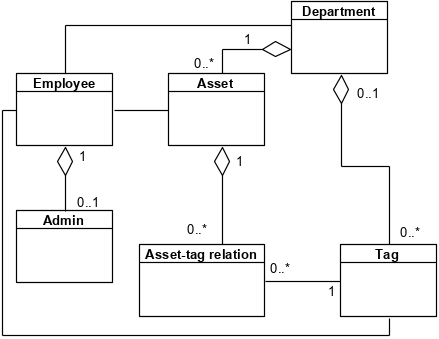
\includegraphics[width=0.8\textwidth]{figures/ClassDiagrams/Class_activity_class_diagram.png}
    \caption{Class diagram of the classes in the problem domain.}
    \label{fig:FirstPDClassDiagram}
\end{figure}

As described in \autoref{sc:classes}, there are six different relevant classes in the problem domain. These classes are: \textit{Employee}, \textit{Admin}, \textit{Department}, \textit{Asset}, \textit{Tag}, and \textit{Asset-tag relation}. The relations between these have been explained below.
\par

The \textit{Employee} class is an aggregation of the \textit{Admin} class. The structure created by this connection is a role pattern with only one role. The pattern makes it possible for an employee to possess the role of \textit{Admin} dynamically.
\par

The \textit{Asset} aggregates a number of \textit{Asset-tag relation}s. On top of this, every asset belongs to one department.
\par

The \textit{Employee} class has a association to the \textit{Asset}, \textit{Department}, and \textit{Tag} classes, as they can see the information on an asset and search for through them based on tags and/or departments. The \textit{Admin} class is a role of the \textit{Employee} class. This means that the functionality kept in the \textit{Admin} class will be available to the employees who have the role of admin.
\par

The \textit{Asset-tag relation} class is created to handle the relation between the \textit{Asset} and \textit{Tag} classes. The \textit{Asset} class aggregates it, as an asset the tags exists only as an addition to the assets. It has been added, as multiple assets can be tagged with the same tag and an asset can have multiple tags. The association to the \textit{Tag} class originates from the relation pattern. An instance of the \textit{Asset-tag relation} class always connects one asset and one tag, but both the \textit{Tag} and \textit{Asset} classes can be part of mulitple asset-tag relations.
\par

With the classes of the problem domain and their interconnecting relations described, the behaviour of the classes can be examined.

% Behavior activity
\section{Behavior} \label{sc:behavoir}
In the following section, the behavior of each class will be examined. A deeper understanding of these behaviours will be achieved through state chart diagrams.
\\\\

\large{\textbf{Asset}}
\begin{figure}[H]
    \centering
    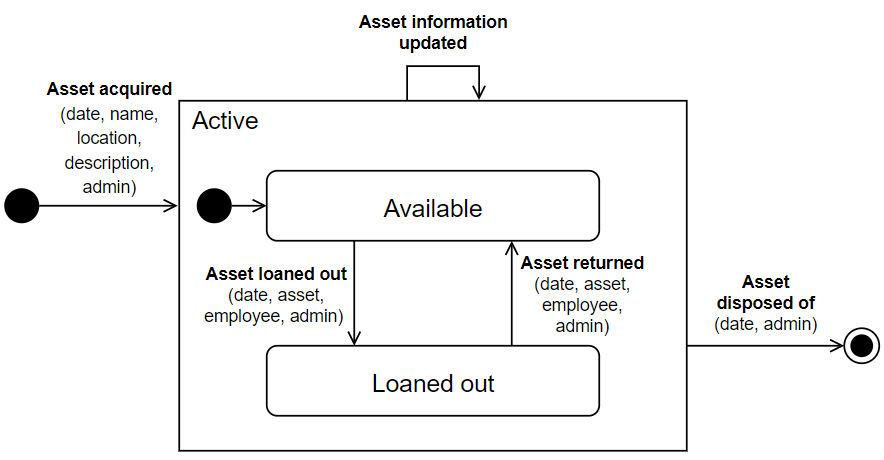
\includegraphics[width=1\textwidth]{figures/StateCharts/Asset_state_chart.png}
    \caption{State chart diagram for the \textbf{Asset} class}
    \label{fig:asset_statechart}
\end{figure}

An object of the \textit{Asset} class is created when an asset is acquired. At first, its state is \textbf{Available}, and when the asset is loaned out to an employee, it changes state to \textbf{Loaned out}. From any of these two states, the asset can be disposed of and removed from the problem domain. Being loaned out will, in the system, simply consist of the asset being tagged with an employee, and the return of the asset will be removing this relation. The information on the asset, not including the tags attached to it, can be updated at all times during its life cycle in the system, and can occur multiple times.
\\\\

\large{\textbf{Employee}}
\begin{figure}[H]
    \centering
    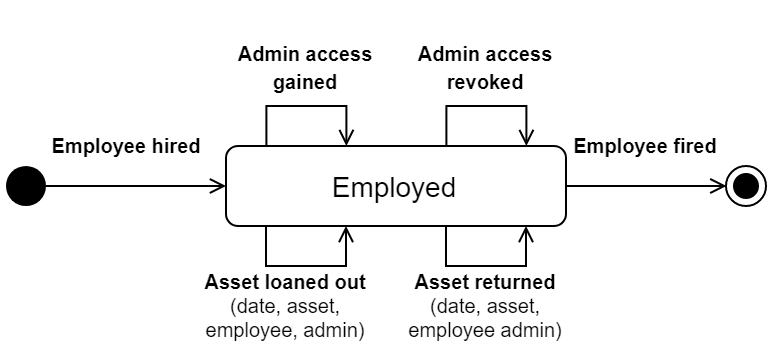
\includegraphics[width=0.8\textwidth]{figures/StateCharts/StateChart_Employee.png}
    \caption{State chart diagram for the \textbf{Employee} class}
    \label{fig:employee_statechart}
\end{figure}

An \textit{Employee} object is created when a person is hired at the zoo and gains the status employed. An employee can be granted admin access, which can later be revoked. An employee can also borrow an asset and return it later. The employee object ceases to exist when the person is fired. The event of returning an asset can only happen when the employee has borrowed the given asset, but an employee can borrow multiple assets at a time, hence both events are iterations.\\
The employee can be granted admin access multiple times during the employment but of course, the access can only be revoked after the access has been granted. Both things can happen multiple times and are therefore iterations. These two events also mark the initialization and end of an admin.
\\\\

\large{\textbf{Admin}}
\begin{figure}[H]
    \centering
    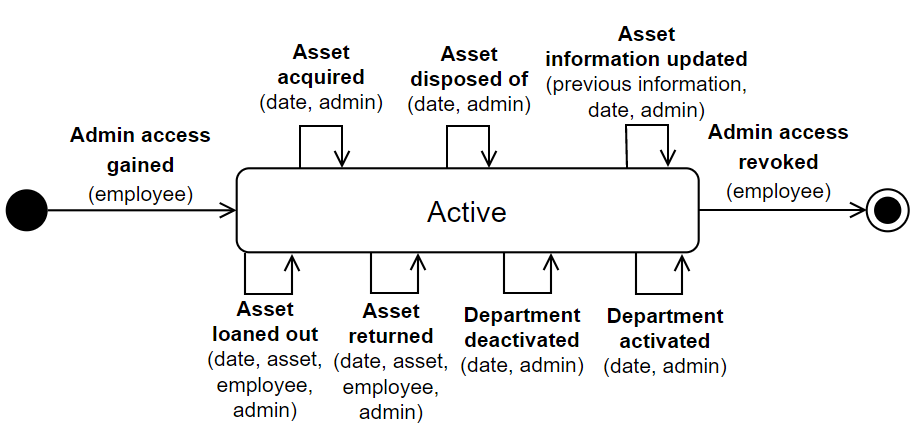
\includegraphics[width=0.8\textwidth]{figures/StateCharts/Admin_state_chart.png}
    \caption{State chart diagram for the \textbf{Admin} class}
    \label{fig:admin_statechart}
\end{figure}

The \textit{Admin} object is created when an employee is granted admin access. As an admin, the employee is responsible for loaning out assets to other employees and receiving the assets when they are returned. The admin will also be responsible for adding tags, assets, activating departments, and maintaining these elements by updating and removing them. The admin object is terminated when the employee's admin access is revoked.
\\\\

\large{\textbf{Tag}}
\begin{figure}[H]
    \centering
    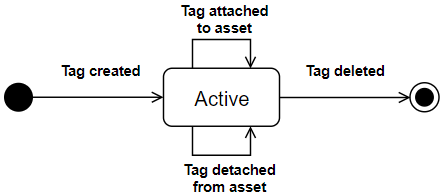
\includegraphics[width=0.6\textwidth]{figures/StateCharts/Tag_state_chart.png}
    \caption{State chart diagram for the \textbf{Tag} class}
    \label{fig:loan_statechart}
\end{figure}

An object of the \textit{Tag} class is created by an admin and can be attached to and detached from assets multiple times during its life cycle. The tag is terminated when an admin deletes it from the system.
\par

With the behaviours of the classes described, the problem domain has been analysed. The following section will sum up the results of the analysis.

% \large{\textbf{Loan}}
% \begin{figure}[H]
%     \centering
%     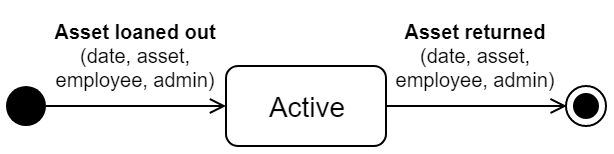
\includegraphics[width=0.8\textwidth]{figures/StateChart_Loan.png}
%     \caption{State chart diagram for the \textbf{Loan} class}
%     \label{fig:loan_statechart}
% \end{figure}

% A \textbf{Loan} object is created when an asset is loaned out and seizes to exist when the asset is returned.
% \newline\par
% With the behaviours of the classes described, the problem domain has been analysed. The following section will sum up the results of the analysis.

% Summary
\section{Summary} \label{ssc:pd_summary}
This chapter has discussed and analysed the different classes and events within the problem domain, as well as the structure and behavior of these. This has given an understanding of the interactions of the objects and an overview of the involved classes and events. The \textit{Tag} class has been added to the problem domain based on dialog with Aalborg Zoo, and the class has handled the loan of an asset to an employee, as well as improving the organizing of assets. The class diagram (see \autoref{fig:FirstPDClassDiagram}) depicts the classes that will form the core of the system and the connections between these. The event table (see \autoref{tab:events}) has listed all the initial events needed in the system to ensure the wanted functionality. Lastly the state charts of the classes (see \autoref{sc:behavoir}) have given an understanding of how the different classes behave and how they participate in different events.
\par

The overview, derived from these elements, has been used as a foundation for the system design and a better understanding of the application domain, which will be analysed in the following chapter..\\


%%%%%%%%%%%%%%%%%%%%%%%%%%%%%%%%%%%%%%%%%%%%%%%%%%%%%%%%%%%%%%%
% Application Domain Analysis
%%%%%%%%%%%%%%%%%%%%%%%%%%%%%%%%%%%%%%%%%%%%%%%%%%%%%%%%%%%%%%%
\chapter{Application Domain Analysis} \label{ch:applicationdomain}
In this chapter, the application domain has been analysed. This analysis involves the different actors, whom the system will be designed to interact with, and the different use cases these actors will go through as they use the system. The use cases have been constructed based on the requirements and the system definition, and make up a basis for the design of the interface and functionality of the system. Based on these, a functions list has been constructed.
\par
To sufficiently describe the needed functionality of the system, the usage of the system has been analysed. This description will be used to facilitate the design of the system and to ensure that it accommodates the way the actors will interact with it.

% Usage activity
\section{Usage}\label{sc:usage}
Within this section, the usage of the system, which include a list of actors and relevant use cases, has been analysed. This part of the application domain is important to understand, in order to create a satisfactory user experience and offer all the relevant functionality in the finished system. Firstly, the actors and use cases have been identified, described, and connected in an actor table.
\subsection{Actors} \label{scc:actors}
The actors in the application domain include the employees and admins. The differentiation of the two is made, because the admin has access to specific functionality and pages within the system, which are not available to the employee. As mentioned in the previous chapter, the admin is a role which an employee can take. This means that an admin has the same abilities as the employee as well as the extra functionalities the role provides.
\par
The descriptions of the actors include their level of experience with similar systems, their goals for using the system, and examples of the actor.

\fancyLayout{actor}{Admin}
    {Specification of the \textit{admin} actor.}
    {actor:admin}
    {
        \textbf{Goal:} The \textit{admin} manages the system. The \textit{admin's} basic goal is to keep track of the company assets.
        \vskip 0.2cm
        
        \textbf{Characteristics:} The \textit{admin} is the primary user of the system and is the only actor who can change anything regarding the assets in the system. They are experienced with using enterprise systems and handling the assets of their department.
        \vskip 0.2cm
        
        \textbf{Example:} This \textit{admin} is used to organising large quantities of assets, and sees the asset management system as a supplement to their organisational tools.
    }

The admin is, as mentioned, the primary user of the system and accommodating their needs has been of highest importance, when it comes to accommodating actor needs.

\fancyLayout{actor}{Employee}
    {Specification of the \textit{employee} actor.}
    {actor:employee}
    {
        \textbf{Goal:} The \textit{Employee} can borrow the company assets. They have a need for borrowing assets that are relevant to their work.
        \vskip 0.2cm
        
        \textbf{Characteristics:} The \textit{Employee} is the secondary user of the system. They can only borrow and view assets within the system. They have varying degrees of technical competence.
        \vskip 0.2cm
        
        \textbf{Examples:} \textit{Employee A} is familiar with computer systems and has no trouble finding their way around the asset management system.
        \vskip 0.1cm
        \textit{Employee B} is less experienced with computer systems and is more comfortable talking directly to the admin instead of using the system themselves. 
    }
As a secondary user of the system, the needs of the employee will have less priority than the needs of the admin.
\subsection{Use cases}\label{ssc:usecases}
The following use cases have been derived from the understanding of the problem domain and actors described in the previous sections. The following description of the use cases include how the interactions with the system will take place, which actors are involved, and which functions are called within the system to complete the actions.
\par
In addition to the already described interactions stated in the system definition, the interviews with Aalborg Zoo have let to the use case of an admin printing out a report of assets from the system. The report can consist of all or some of the assets in the system and will be saved as a separate file on the admins computer.
% \par
% Each use case has been described and is followed by a diagram of the interaction.
\newline

\fancyLayout{use_case}{Add an asset}
    {Use case for adding an asset}
    {use_case:add_an_asset}
    {
        \textbf{Use Case:} Adding an asset is done by an admin. The admin goes to the add asset page, attaches the relevant tags, and fills in the relevant information about the asset. The admin then saves the asset in the system and it becomes visible to all employees.
    
        \vskip 0.2cm
        
        \textbf{Objects:} Admin, Asset
        
        \vskip 0.2cm
        
        \textbf{Functions:} Add asset
    }

\begin{figure}[H]
    \centering
    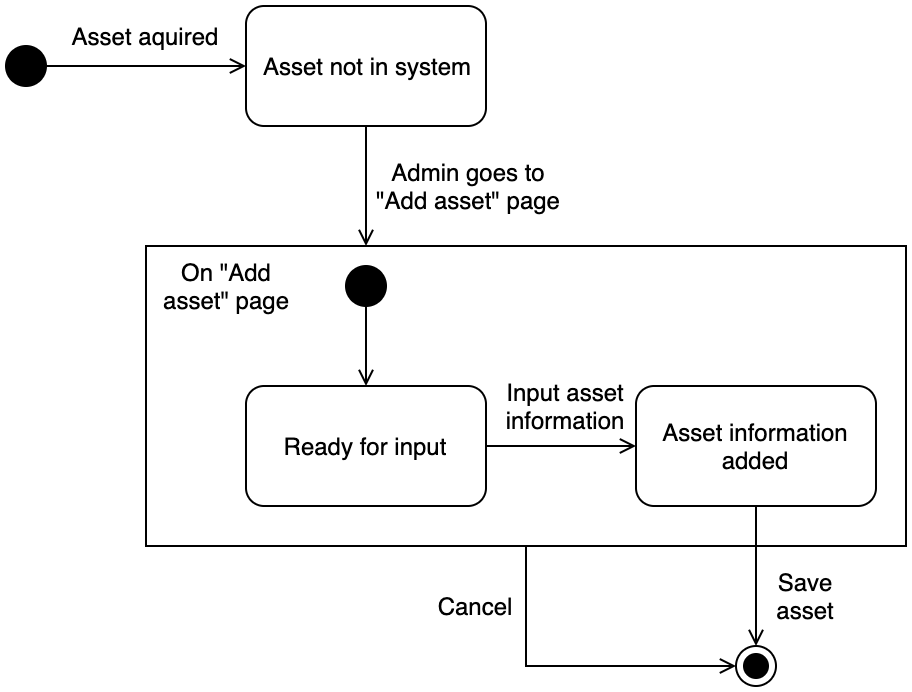
\includegraphics[width=0.8\textwidth]{figures/UseCases/UC_Add_asset.png}
    \caption{User interface state chart diagram for adding an asset}
    \label{fig:add_asset_statechart}
\end{figure}

\newpage

\fancyLayout{use_case}{Loan out an asset}
    {Use case for loaning out an asset}
    {use_case:loan_out_an_asset}
    {
        \textbf{Use Case:} Loaning out an asset is done by an admin, whom an employee contacts, when they want to borrow the given asset. The admin goes to the page of the given asset and attaches the employee's tag to it. The admin then hands over the asset to the employee.
    
        \vskip 0.2cm
        
        \textbf{Objects:} Admin, Asset, Employee, Tag
        
        \vskip 0.2cm
        
        \textbf{Functions:} Asset loaned out, Tag attached to asset
    }
 
\begin{figure}[H]
    \centering
    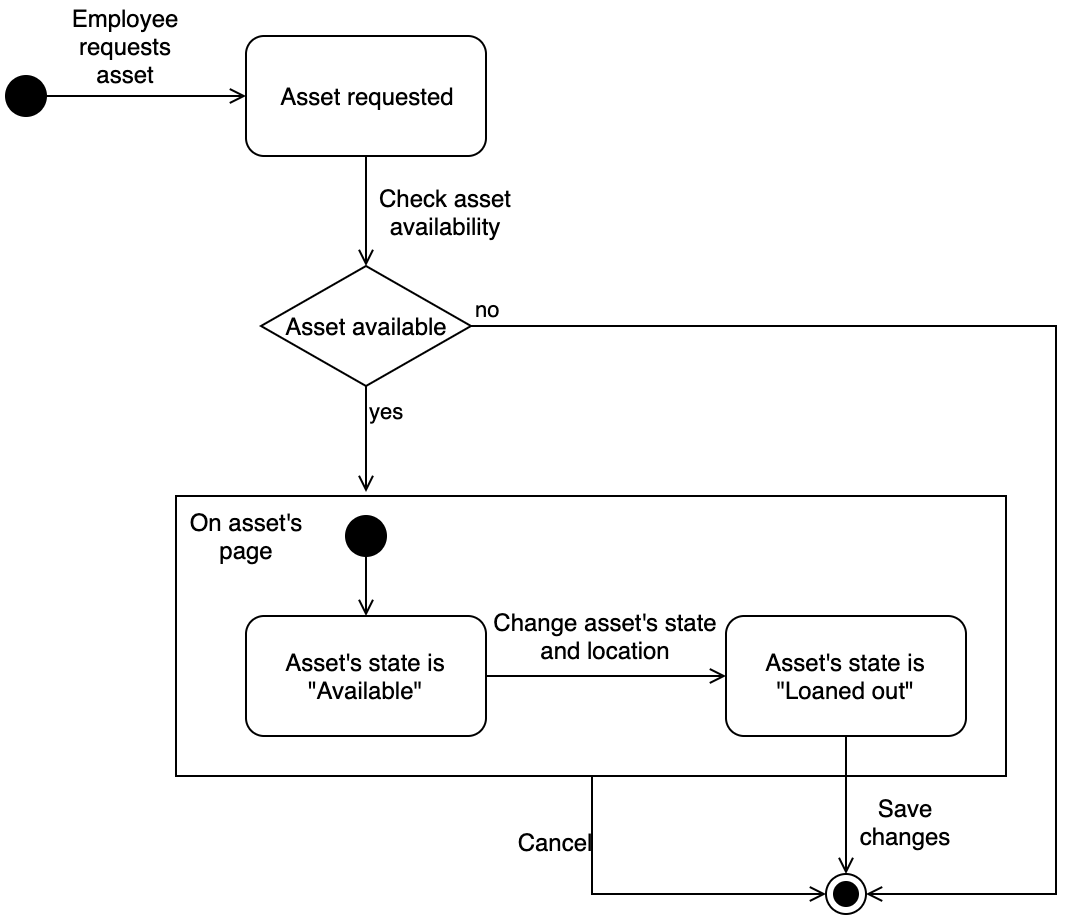
\includegraphics[width=0.8\textwidth]{figures/UseCases/UC_Loan_out_asset.png}
    \caption{User interface state chart diagram for loaning out an asset}
    \label{fig:loan_out_asse_statechart}
\end{figure}
\todo{Update diagram}
 
\fancyLayout{use_case}{Return an asset}
    {Use case for returning an asset}
    {use_case:return_an_asset}
    {
        \textbf{Use Case:} When an asset is being returned by an employee, it is handed over to an admin. The admin then goes to the page of the given asset and detaches the tag of the employee from the asset.
    
        \vskip 0.2cm
        
        \textbf{Objects:} Admin, Asset, Employee, Tag
        
        \vskip 0.2cm
        
        \textbf{Functions:} Update asset information, Tag detached from asset
    }
    
\begin{figure}[H]
    \centering
    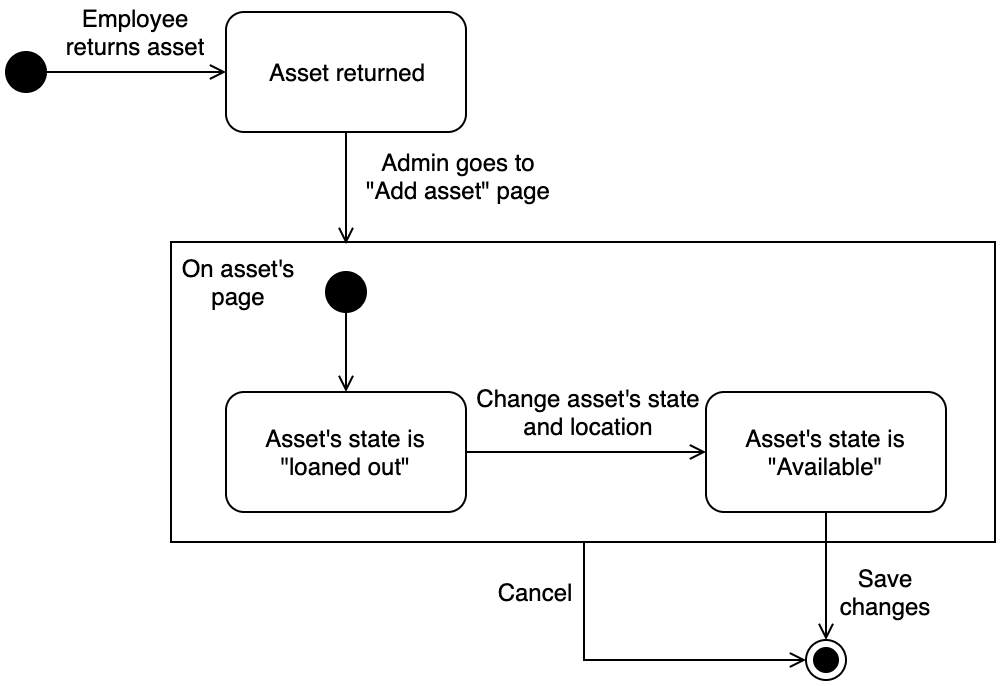
\includegraphics[width=0.8\textwidth]{figures/UseCases/UC_Return_asset.png}
    \caption{User interface state chart diagram for returning an asset}
    \label{fig:return_asset_statechart}
\end{figure}
\todo[inline]{Update diagram}

\fancyLayout{use_case}{Change the information of an asset}
    {Use case for changing the information of an asset}
    {use_case:changing_the_information_about_an_asset}
    {
        \textbf{Use Case:} If one of the states of an asset changes, the changed data should be updated in the system by an admin. These changes could be things such as the asset going from working to being broken or being updated to a new operation system. To update the asset's information, the admin goes to the given asset's page, can then press the edit button, and change the outdated data to comply with the new state of the asset in the problem domain.
    
        \vskip 0.2cm
        
        \textbf{Objects:} Admin, Asset
        
        \vskip 0.2cm
        
        \textbf{Functions:} Search for asset, Update asset information, View asset
    }
    
\begin{figure}[H]
    \centering
    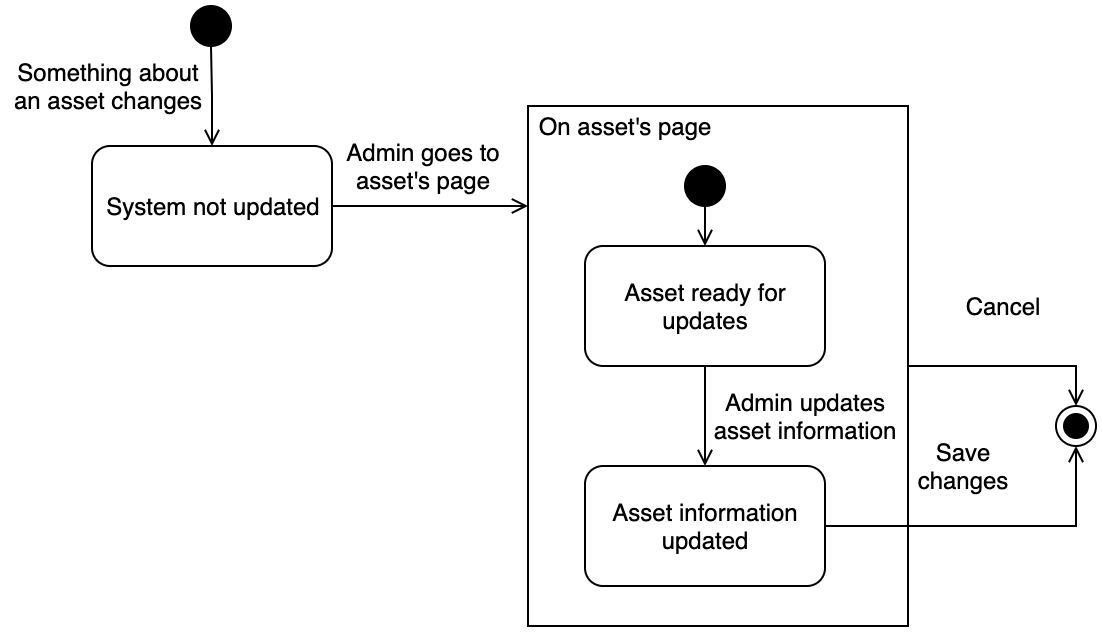
\includegraphics[width=0.8\textwidth]{figures/UseCases/UC_Change_asset.png}
    \caption{User interface state chart diagram for changing an asset}
    \label{fig:edit_asset_statechart}
\end{figure}

\newpage

\fancyLayout{use_case}{Remove an asset}
    {Use case for removing an asset}
    {use_case:remove_an_asset}
    {
        \textbf{Use Case:} When an asset is no longer needed within the problem domain, it is discarded. This is handled in the system by an admin. The admin goes to the page of the given asset and deletes it from the system. The asset is then removed from the system and is no longer visible to any of the employees.
    
        \vskip 0.2cm
        
        \textbf{Objects:} Admin, Asset, Employee
        
        \vskip 0.2cm
        
        \textbf{Functions:} Remove asset
    }

\begin{figure}[H]
    \centering
    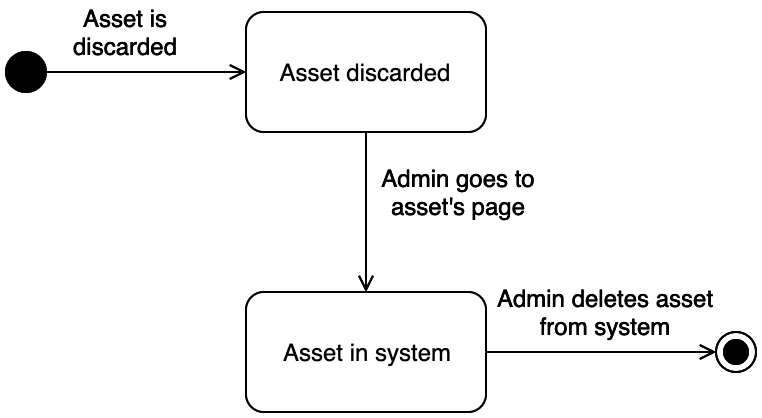
\includegraphics[width=0.8\textwidth]{figures/UseCases/UC_Remove_asset.png}
    \caption{User interface state chart diagram for removing an asset}
    \label{fig:remove_asset_statechart}
\end{figure}

\newpage

\fancyLayout{use_case}{Search for an asset}
    {Use case for searching for an asset}
    {use_case:search_for_an_asset}
    {
        \textbf{Use Case:} If a user wants information about a specific asset, this can be achieved by going to the search page and entering some information about the asset in the search field. The system then returns a list of assets complying with the search query. The user can then choose the desired asset.
    
        \vskip 0.2cm
        
        \textbf{Objects:} Admin, Asset, Employee
        
        \vskip 0.2cm
        
        \textbf{Functions:} Search for asset, View asset
    }

\begin{figure}[H]
    \centering
    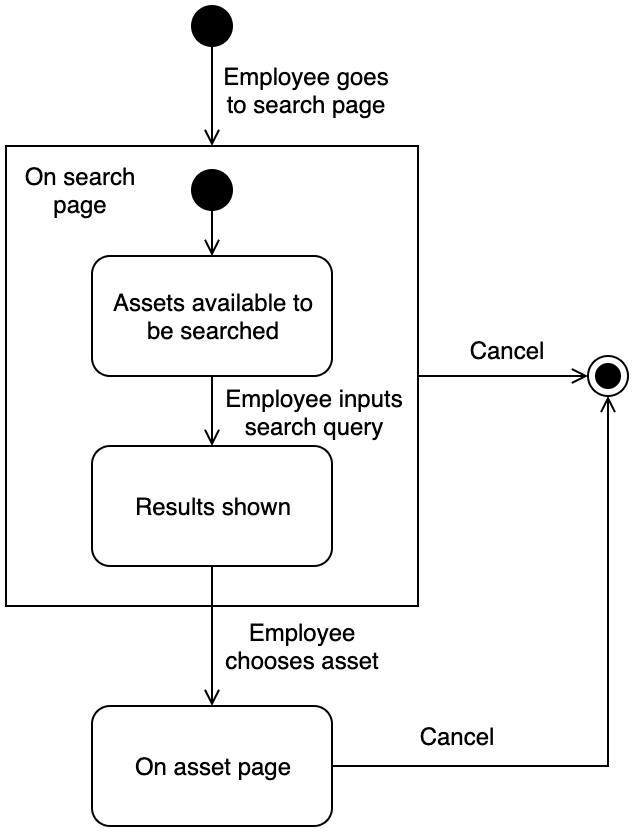
\includegraphics[width=0.6\textwidth]{figures/UseCases/UC_Search_asset.png}
    \caption{User interface state chart diagram for searching for an asset}
    \label{fig:search_asset_statechart}
\end{figure}

\fancyLayout{use_case}{Print a report of assets}
    {Use case for printing a report of assets}
    {use_case:print_a_report_of_assets}
    {
        \textbf{Use Case:} As the number of assets in the system increases, an admin might want to retrieve a number of assets from the system. The admin goes to the asset list page, selects the assets they want to retrieve from the system and presses the print button. The system then generates a file containing information about the selected assets and saves it on the admin's computer.
    
        \vskip 0.2cm
        
        \textbf{Objects:} Admin, Asset
        
        \vskip 0.2cm
        
        \textbf{Functions:} Export report
    }

\begin{figure}[H]
    \centering
    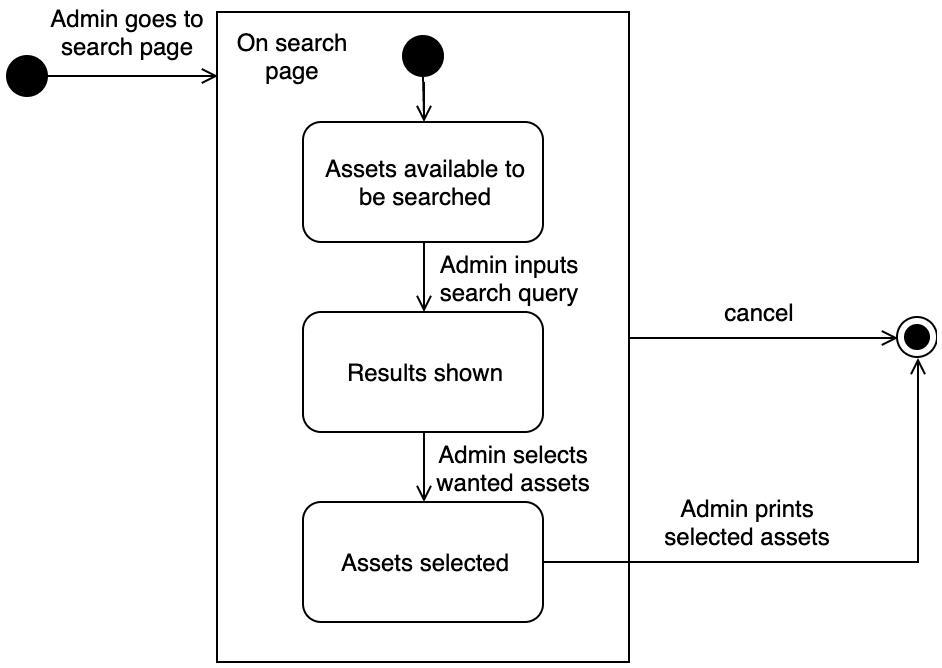
\includegraphics[width=0.8\textwidth]{figures/UseCases/UC_Print_report.png}
    \caption{User interface state chart diagram for printing out a report}
    \label{fig:print_report_statechart}
\end{figure}

\fancyLayout{use_case}{Comment on an asset}
    {Use case for commenting on an asset}
    {use_case:commenting_on_an_asset}
    {
        \textbf{Use Case:} A user might have a comment regarding an asset, such as an issue they have had with it or suggestions for improvements. To share this information with other users, they can go to the page of the asset and add a comment to it. This comment will be visible to all users.
    
        \vskip 0.2cm
        
        \textbf{Objects:} Admin, Asset, Employee
        
        \vskip 0.2cm
        
        \textbf{Functions:} Add comment to asset, Search for asset, View Asset
    }

\begin{figure}[H]
    \centering
    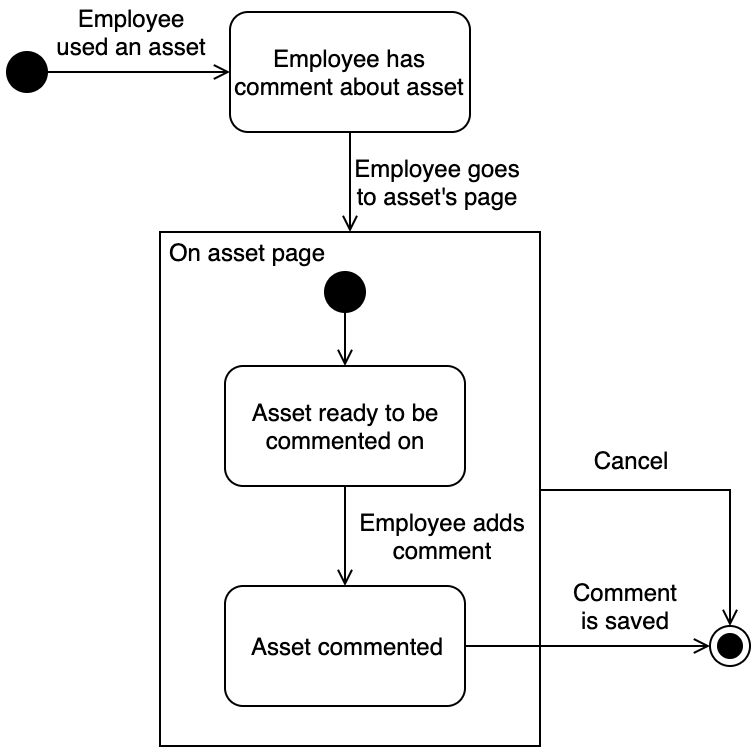
\includegraphics[width=0.8\textwidth]{figures/UseCases/UC_Add_comment.png}
    \caption{User interface state chart diagram for adding a comment to an asset}
    \label{fig:add_comment_statechart}
\end{figure}

These are the relevant use cases for managing the assets. The use cases have been placed in an actor table with the two previously described actors in order to illustrate the connections between these.

\begin{table}[H]
    \centering
    % \hrule
    \vspace{0.2cm}
    \hspace{6cm} \vspace{0.6cm} \textbf{Actors}
    \begin{tabular}{p{0.5\textwidth} || p{0.2\textwidth} p{0.2\textwidth}}
        \textbf{Use cases} & Admin & Employee \vspace{0.2cm}\\
        \hline \hline
        Add an asset & \hspace{0.34cm} \checkmark & \\
        \hline
        Loan out an asset & \hspace{0.34cm} \checkmark & \hspace{0.6cm} \checkmark \\
        \hline
        Return an asset & \hspace{0.34cm} \checkmark & \hspace{0.6cm} \checkmark \\
        \hline
        Change the information about an asset & \hspace{0.34cm} \checkmark & \\
        \hline
        Remove an asset & \hspace{0.34cm} \checkmark & \\
        \hline
        Search for an asset & \hspace{0.34cm} \checkmark & \hspace{0.6cm} \checkmark \\
        \hline
        Print a report of assets & \hspace{0.34cm} \checkmark & \\
        \hline
        Comment an asset & \hspace{0.34cm} \checkmark & \hspace{0.6cm} \checkmark\\
    \end{tabular}
    \vspace{0.2cm}
    % \hrule
    \vspace{0.2cm}
    \caption{Actor table of the relations between actors and use cases.}
    \label{tab:actor_table}
\end{table}

As the actor table above shows, the admin takes part in every use case. This can be explained by the way the system will be used. The system should function almost like an interface to a database, so it makes sense that the admin will be involved in all the changes made to the system and the database.\\

The defined use cases have then been used to extract relevant functions and, later in the report, construct the user interface (see \autoref{ch:ui_design}). For most of these use cases, the system should limit the access of the employees without admin status, which has resulted in two additional functions, \textit{Authenticate user} and \textit{Check access level}. These functions are used to guarantee that parts of the system is only accessible to employees with admin status and are executed on login and most of the described use cases above.
\par
The functions discovered in this section have been analysed and described in the following section.

% Function activity
\section{Function activity}\label{sc:function}
Based on the use cases, it is possible to determine the functions necessary for the system to adequately fulfill the requirements. These functions have been classified by their type and complexity in the following function list. The complex functions have then been further split into smaller functions to explain their processes. This is done following the functions analysis and the complexity definitions from \cite[chap 7]{OOAD}. The complexity definitions are:
\begin{itemize}
    \item Simple: Sets or reads the value of an attribute in an existing object.
    \item Medium: Creates a new object and connects it by object structure(s) to other objects.
    \item Complex: Reads from or creates several objects (from different classes).
\end{itemize}
With these definitions, the following function table has been constructed.

\begin{table}[H]
\centering
    \begin{tabular}{|l|l|l|}
        \hline
        \textbf{Function} & \textbf{Complexity} & \textbf{Type} \\
        \hline
        \hline
        Add asset & Complex & Update\\
        \hline
        Remove asset & Simple & Update\\
        \hline
        Update asset information & Complex & Update\\
        \hline
        Comment asset & Medium & Update\\
        \hline
        Search for asset & Medium & Compute/Read\\
        \hline
        View asset & Simple & Read\\
        \hline
        Add department & Simple & Update\\
        \hline
        Remove department & Simple & Update\\
        \hline
        Authenticate user & Simple & Read\\
        \hline
        Check access level & Simple & Read\\
        \hline
        Export report & Complex & Compute/Read\\
        \hline
        Attach tag & Simple & Update\\
        \hline
        Detach tag & Simple & Update\\
        \hline
    \end{tabular}
\caption{Function table showing all the different top-level functions as well as their complexity and type.}\label{tab:functions}
\end{table}

The function table (see \autoref{tab:functions}) contains multiple complex functions. As mentioned earlier, these functions have been further split into smaller functions to better understand the operations.


\fancyLayout
    {function}
    {Add asset}
    {The table shows the different functions involved in adding an asset as well as their complexity.}
    {function:add_asset}
    {
        \centering
        \begin{tabular}{|l|l|l|}
            \hline
            \textbf{Function} & \textbf{Complexity} & \textbf{Type}\\
            \hline
            \hline
            Add relevant information about the asset & Simple & Update \\
            \hline
            Save Asset to model & Medium & Update \\
            \hline
            Update connections to tags & Medium & Update\\
            \hline
        \end{tabular}
}

The \textit{Add asset} function consists of three smaller functions, as seen in \autoref{function:add_asset}. When adding an asset, first the admin enters the relevant information, which is then saved with the asset to the model. Lastly, the \textit{Asset-tag relation}s connected to the asset are updated. This last step possibly creates and deletes \textit{Asset-tag relation}s between the asset and the relevant tags.

\fancyLayout
    {function}
    {Update asset information}
    {The table shows the different functions involved in updating an assets information.}
    {function:update_asset_information}
    {
        \centering
        \begin{tabular}{|l|l|l|}
            \hline
            \textbf{Function} & \textbf{Complexity} & \textbf{Type}\\
            \hline
            \hline
            Load asset from model & Simple & Read \\
            \hline
            Update relevant information about the asset & Simple & Update \\
            \hline
            Save asset to model & Medium & Update \\
            \hline
            Update connections to tags & Medium & Update\\
            \hline
        \end{tabular}
}

The \textit{update asset information} function is made up of the smaller functions, as shown in \autoref{function:update_asset_information}, which will be executed in the shown order. First, the asset is loaded from the model and formatted as an asset in the system. Then the changes to the information is applied to the asset. The asset is then saved to the model with the changes and its connections to tags are updated. Just as the \textit{Add asset} function, the last step possibly creates and deletes \textit{Asset-tag relation}s between the asset and the relevant tags.

\fancyLayout
    {function}
    {Export report}
    {The table shows the different functions involved in exporting a report.}
    {function:export_report}
    {
        \centering
        \begin{tabular}{|l|l|l|}
            \hline
            \textbf{Function} & \textbf{Complexity} & \textbf{Type}\\
            \hline
            \hline
            Load assets to be included & Simple & Update \\
            \hline
            Create entries & Simple & Update \\
            \hline
            Build report & Simple & Update \\
            \hline
            Export to CSV-format & Medium & Compute \\
            \hline
        \end{tabular}
}

The \textit{export report} function involves the four smaller functions listed in \autoref{function:export_report}, happening in order. The first step is that the selected assets are loaded. Then report entries are created based on the assets, which are then added to the report. Finally the report is exported to the admin's computer formatted as a Comma Separated Values (CSV) file.
\par
This concludes the analysis of functions. The understanding of the users and functions has been used in the following section as a basis for the interface.
\section{Functions}\label{sc:functions}

This section will present the functions in the system. Table \ref{tab:functions} shows all the top-level functions that the system will be able to perform. All the tables describing functions have columns with the name of the function, the complexity and the type of function.

\begin{table}[H]
\centering
%\resizebox{\textwidth}{!}{%
    \begin{tabular}{|l|l|l|}
        \hline
        \textbf{Function} & \textbf{Complexity} & \textbf{Type} \\
        \hline
        \hline
        Add asset & Complex & Update\\
        \hline
        Remove asset & Medium & Update\\
        \hline
        Edit asset & Complex & Update\\
        \hline
        Search asset & Medium & Compute/Read\\
        \hline
        View asset & Simple & Read\\
        \hline
        Add tag & Simple & Update\\
        \hline
        Remove tag & Medium & Update\\
        \hline
        Rename tag & Simple & Update\\
        \hline
        Tag asset & Simple & Update\\
        \hline
        Untag asset & Simple & Update\\
        \hline
        Authenticate user & Simple & Read\\
        \hline
        Check access level & Simple & Read\\
        \hline
        Export report & Complex & Compute/Read\\
        \hline
        Export log & Complex & Compute/Read\\
        \hline
    
    \end{tabular}
%}
\caption{Table showing all the different top-level functions as well as their complexity and type.}\label{tab:functions}
\end{table}

\par

Table \ref{tab:functions} contains several functions rated complex. These functions have been divided into several smaller functions, with a lower complexity.
% Beskriver hvorfor det er gjort, ved ikke om det skal med, men det er god fyldertekst
This is done in order to divide the complex problems into smaller problems, which are easier to implement. 
 
\begin{center}
    \textbf{Adding an asset}
\end{center}

% Add asset table
\begin{table}[H]
\centering
%\resizebox{\textwidth}{!}
\caption{Table showing the different functions involved in adding an asset along with their complexity and type.}\label{tab:AddAssetFunctions}
\end{table}

\par

\begin{center}
    \textbf{Editing an asset}
\end{center}

% Edit Asset Table
\begin{table}[H]
\centering
%\resizebox{\textwidth}{!}
\caption{Table showing the different functions involved in editing an asset along with their complexity and type.}\label{tab:EditAssetFunctions}
\end{table}

\par

% \begin{center}
%     \textbf{Adding a template}
% \end{center}

% % Add template table 
% \begin{table}[H]
% \centering
% %\resizebox{\textwidth}{!}{%
%     \begin{tabular}{|l|l|l|}
%         \hline
%         \textbf{Function} & \textbf{Complexity} & \textbf{Type} \\
%         \hline
%         \hline
%         Add Field & Simple & Update\\
%         \hline
%         Save Template & Medium & Update\\
%         \hline
        
%     \end{tabular}
% %}
% \caption{Table showing the different functions involved in adding a template along with their complexity and type.}\label{tab:AddTemplateFunctions}
% \end{table}

% \par

% \begin{center}
%     \textbf{Editing a template}
% \end{center}

% % Edit template table
% \begin{table}[H]
% \centering
% %\resizebox{\textwidth}{!}{%
%     \begin{tabular}{|l|l|l|}
%         \hline
%         \textbf{Function} & \textbf{Complexity} & \textbf{Type} \\
%         \hline
%         \hline
%         Add Field & Simple & Update\\
%         \hline
%         Remove Field & Simple & Update\\
%         \hline
%         Load Template & Medium & Read\\
%         \hline
%         Save Template & Medium & Update\\
%         \hline
        
%     \end{tabular}
% %}
% \caption{Table showing the different functions involved in editing a template along with their complexity and type.}\label{tab:EditTemplateFunctions}
% \end{table}

% \par

\begin{center}
    \textbf{Exporting a report}
\end{center}

% Export report table
\begin{table}[H]
\centering
%\resizebox{\textwidth}{!}
\caption{Table showing the different functions involved in exporting a report along with their complexity and type.}\label{tab:ExportReportFunctions}
\end{table}

% User interface
\section{User interface}\label{sc:userinterface}
% intro intro

\begin{figure}[H]
    \centering
    \frame{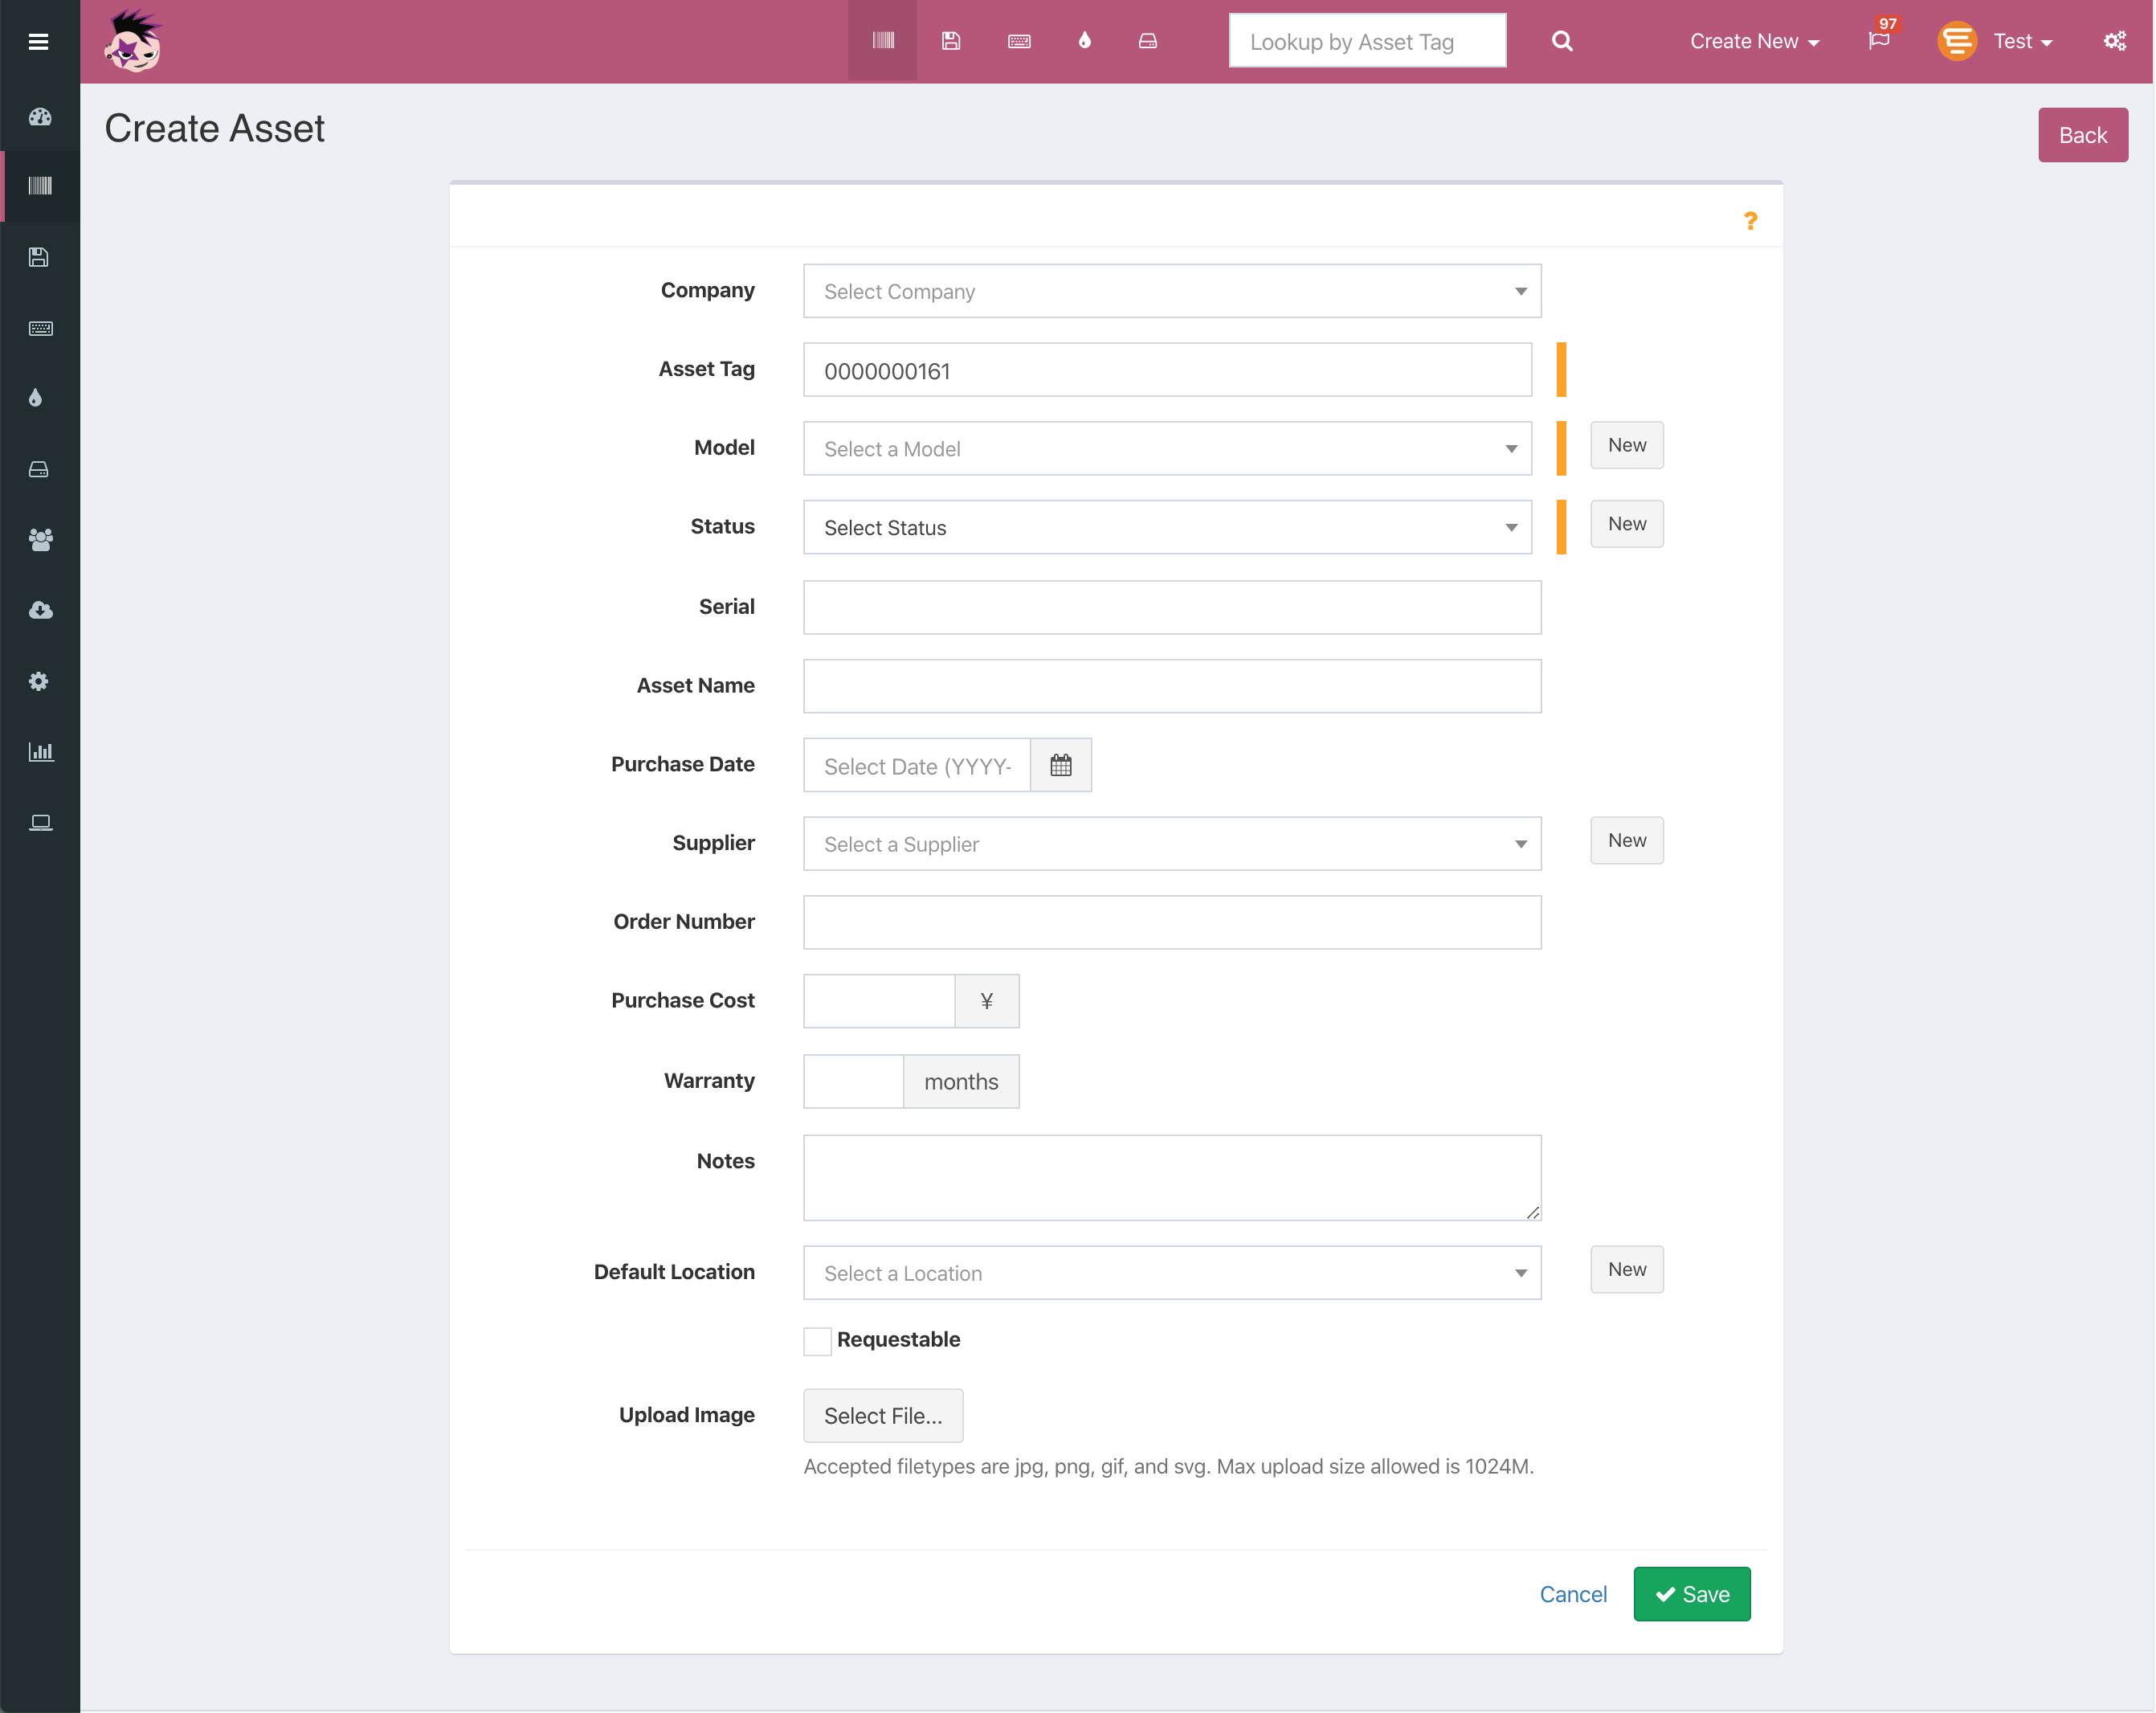
\includegraphics[width=0.9\textwidth]{figures/other-systems/snipeitapp-create-asset-ui-screenshot.png}}
    \caption{Caption}
    \label{fig:too}
\end{figure}


The user interface is following the KISS-principle (Keep It Simple Stupid) and therefore only contains the utmost required interface-elements. As mentioned in \autoref{ch:introduction} and \autoref{ch:problemdefinition} our client needs an easier process of maintaining assets compared to existing solutions on the market. Existing solutions often present the user with a number of fields depending on the category an asset belongs to. This often result in empty and unnecessary fields that are never used. Our approach is based on fields dynamically appearing based on tags added to an asset.

\begin{figure}[H]
    \centering
    \frame{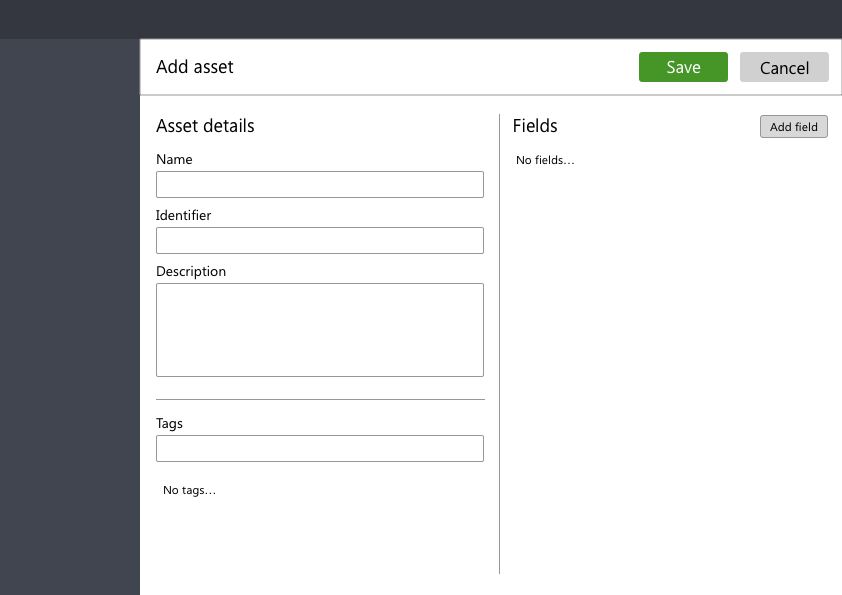
\includegraphics[width=0.9\textwidth]{figures/wireframes/add-asset-no-tags.png}}
    \caption{The process of creating a new asset, at this point no tags or custom fields were added, resulting in no fields beside base fields.}
    \label{fig:add-asset-no-tags}
\end{figure}

\begin{figure}[H]
    \centering
    \frame{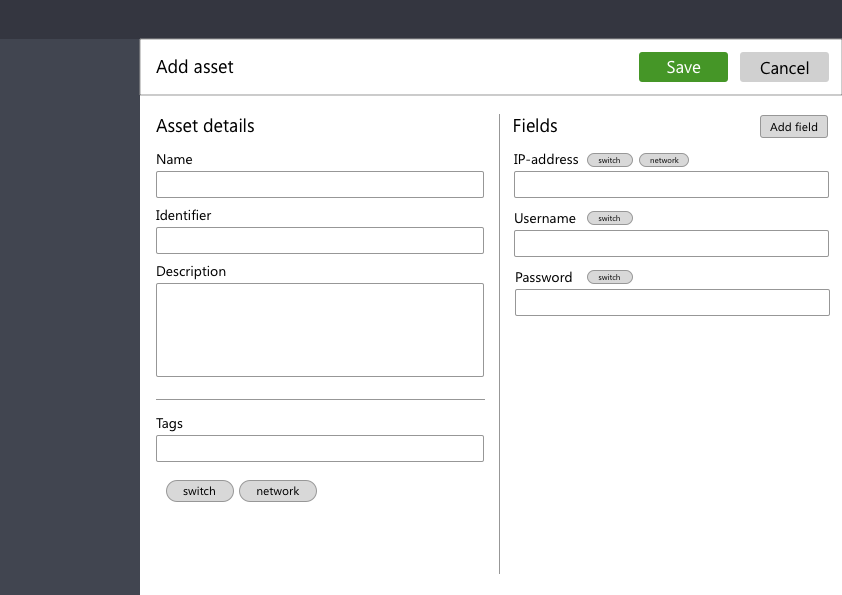
\includegraphics[width=0.9\textwidth]{figures/wireframes/add-asset-with-tags.png}}
    \caption{User interface state chart diagram for searching for an asset}
    \label{fig:add_asset_with_tags}
\end{figure}


\subsection{Employee}
Employees have access to the application and are capable of performing basic operations within the system.

\textbf{Splashscreen:} the first screen visible to the user at application startup 

% Dash / overview page
% Assets list page
% Asset view
% Add comments to asset
% Edit/remove own assets
% Menues?

\subsection{Admin}
Admins are able to do everything an Employee can but their enhanced access make them able to manage system content.

% Add/edit/delete departments
% Add/edit/delete assets
% Add/edit/delete tags
% Add/edit/delete all comments
% Read logs
% Export reports
% Import user data from third-part // Allowing employees access to the system
% 
\section{PACT analysis}\label{sc:PACT}


\textbf{People}:
%(Physiological differences, Psychological differences, Social differences, Domain Expertise)
\begin{itemize}
    \item Morten (IT)
    \item Kasper (IT)
    \item Employees at the zoo
\end{itemize}

\par
No physiological, physiological or social differences to speak of. Morten and Kasper are both IT people, which means they are used to working with computers. However, they have requested the interface to be minimalistic and easy to use, which means most people should be able to use it.
The other employees at the zoo have experience with other computer-based systems through their work.
\par

\textbf{Activities}: \\
%(Purpose of activities to be supported by the system, Temporal aspects, Collaboration, Complexity, Safety criticality, Nature of system content) \\
The system will support registration of assets, and helping users keep track of them. The IT-department adds, edits, updates and removes assets from the system and exports list of assets. They also log changes to the assets and keep track of the assets. On occasion they want a specific asset, which should be easily available to them.
The rest of the employees only use the system to see assets and their current state.
\par

\textbf{Context}: \\
%(Physical, Social, Organizational) \\
The system will be used at Aalborg Zoo, primarily on a desktop or laptop located in the office of the IT department. The laptops might be moved around the premise of the zoo. The software does not contain any elements geared towards any social aspects.
Within Aalborg Zoo the program is developed specifically for the IT department.
\par
 
\textbf{Technology}:
%(That could support users in the domain)
\begin{itemize}
    \item Computer
    \item Barcode scanner
    \item Screen
    \item Mouse
    \item Keyboard
    \item Internet
    \item Database
    \item Active Directory (AD)
\end{itemize}


% Summary
\section{Summary} \label{ssc:ad_summary}
In this chapter, the application domain has been analysed. The different actors that will interact with the system have been identified and a number of use cases have been described in order to better understand the purpose of the system. Based on this, essential system functions have been described, which were used to examine the requirements for the user interface the system. 
\par
The analysis has been used in designing the system architecture in the following chapter.


%%%%%%%%%%%%%%%%%%%%%%%%%%%%%%%%%%%%%%%%%%%%%%%%%%%%%%%%%%%%%%%
% Architectural Design
%%%%%%%%%%%%%%%%%%%%%%%%%%%%%%%%%%%%%%%%%%%%%%%%%%%%%%%%%%%%%%%
\chapter{Architectural Design} \label{ch:architectural_design}
Upon development of the program, more components and subsystems have been added to the system structure. The system has been split into smaller parts to get a better understanding of the components of the system, and a more detailed class diagram has been made. These components will be discussed in the following section.

% Technical Platform
\section{Technical Platform} \label{sc:tech_intro}

\subsection{Database}\label{ssc:tech_database}
MySQL
\subsection{Windows Presentation Platform} \label{ssc:tech_wpf}
Windows Presentation Platform (WPF) is used for all interactions with the user.
\subsection{.NET Core} \label{ssc:tech_core}
???

% Criteria
\section{Criteria} \label{sc:criteria}
% Criteria criteria

\begin{table}[H]
    \centering
    \resizebox{\textwidth}{!}{%
    \begin{tabular}{|l|c|c|c|c|}
        \hline
        \textbf{Criterion} & \textbf{Very important} & \textbf{Important} & \textbf{Less important} & \textbf{Irrelevant} \\
        \hline
        \hline
        Usable & $\pmb{\times}$ & & & \\
        \hline
        Secure & & & $\pmb{\times}$ & \\
        \hline
        Efficient & & & $\pmb{\times}$ & \\
        \hline
        Correct & $\pmb{\times}$ & & & \\
        \hline
        Reliable & & $\pmb{\times}$ & & \\
        \hline
        Maintainable & & $\pmb{\times}$ & & \\
        \hline
        Testable & & & $\pmb{\times}$ & \\
        \hline
        Flexible & $\pmb{\times}$ & & & \\
        \hline
        Comprehensible & & $\pmb{\times}$ & & \\ 
        \hline
        Reuseable & & & & $\pmb{\times}$ \\
        \hline
        Portable & & & & $\pmb{\times}$ \\
        \hline
        Interoperable & & & $\pmb{\times}$ & \\
        \hline
    \end{tabular}
    }
    \caption{Checklist for prioritizing design criteria}
    \label{tab:my_label}
\end{table}

\textbf{Usable:} One of the primary reasons for Aalborg Zoo to get a system developed from scratch, is to get a system that is easy to navigate. Therefore, this is a very important element of the system and the final product. The system is primarily built with usability in focus.

\textbf{Secure:} As the product does not contain any confidential information, security in the system is considered less important. However there is still a minor focus on security, as access to the functions within the program is limited to users with the required permissions.

\textbf{Efficient:} The client has expressed that the efficiency of the system is of little concern, so this criteria is considered less relevant. However, it should still be able to complete the tasks within a reasonable amount of time.

\textbf{Correct:} Aalborg Zoo has given weighted requirements for the system, as seen in \autoref{sc:requirements}. It is very important that the requirements are met upon delivering the finished product. 

\textbf{Reliable:} As part of the heavy focus on the user experience, it is important that the system behaves in a predictable manner, and does this reliably.

\textbf{Maintainable:}
The client has expressed a desire for the program to be maintainable, because they want to maintain the system by themselves. Because they aren't experts in programming, the system should be as easily maintainable as possible, and build on industry standards.

\textbf{Testable:}
As with all other systems, this system should be developed in such a way, that it is testable. This criteria is marked as less important, because it is not the main focus of the project, but it is still regarded as valuable.

\textbf{Flexible:}
The client wants to be able to further develop the system after the product is delivered. Therefore it is very important that it is flexible and without too many dependencies.

\textbf{Comprehensible:}
The system should be comprehensible, as it allows the client to easily add the functionality they need later on. For this reason, this criterion is important.

\textbf{Reusable:}
No part of the system will be used in other systems and therefore, this criterion is irrelevant.

\textbf{Portable:}
The system will only be built for a Windows PC, and for this reason, there is no need for the system to be portable. 

\textbf{Interoperable:}
The system will not communicate with other systems, beside the database component, which means this criterion is less important.

% Component design
\section{Component Architecture} \label{sc:component_architecture}
\begin{figure}[H]
    \centering
    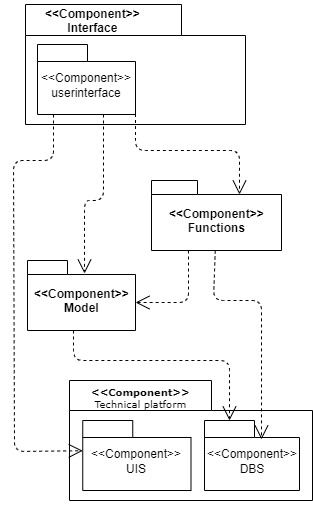
\includegraphics[width=0.6\textwidth]{figures/Componentdiagram.jpg}
    \caption{Component diagram for the Field Component}
    \label{fig:ComponentDesign}
\end{figure}
As seen on \ref{fig:ComponentDesign} the architecture of the system closely resembles the "Generic Architecture Pattern" described in \todo[inline]{Tilføj reference til OOA\&D side 198}.
On the bottom is the database layer, which contains representations of the objects within the program. These representations get converted into accessible and usable objects via the Model layer. The function of the model layer is to convert the representations into objects, which the functions component can utilize and manipulate. Based on the instructions from the interface component, the function layer will manipulate or add objects from the model layer.

% Model component
\section{Model Component} \label{sc:model_component}
Based on the analysis of the problem domain, through the class diagram, event table and state charts. It it possible to create an updated model of the problem domain. 
\par
This is done by specifying the model component mentioned in section \ref{sc:component_architecture}. The result is an updated class diagram, that contains attributes and operations. 

% Tags og andre ting skal introduceres inden dette afsnit
\begin{figure}[H]
    \centering
    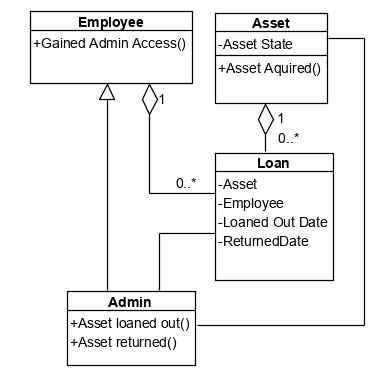
\includegraphics[width=0.8\textwidth]{figures/Model_ComponentV2.PNG}
    \caption{Diagram of the model component}
    \label{fig:ModelComponent}
\end{figure}

As illustrated in figure \ref{fig:ModelComponent} ...

% Function component
\section{Function Component} \label{sc:function_component}

%%%%%%%%%%%%%%%%%%%%%%%%%%%%%%%%%%%%%%%%%%%%%%%%%%%%%%%%%%%%%%%
% Implementation
%%%%%%%%%%%%%%%%%%%%%%%%%%%%%%%%%%%%%%%%%%%%%%%%%%%%%%%%%%%%%%%
\chapter{Implementation}
In this chapter, the implementation of the previously mentioned elements as well as the design patterns used in the system will be discussed.
\par
The following class diagram (see \autoref{fig:CompleteClassDiagram}) illustrates the structure of the central part of the the system being developed. It does not include any classes related to either the UI, the database, or the log, but focuses on how the system models the problem domain. 

\begin{figure}[H]
    \centering
    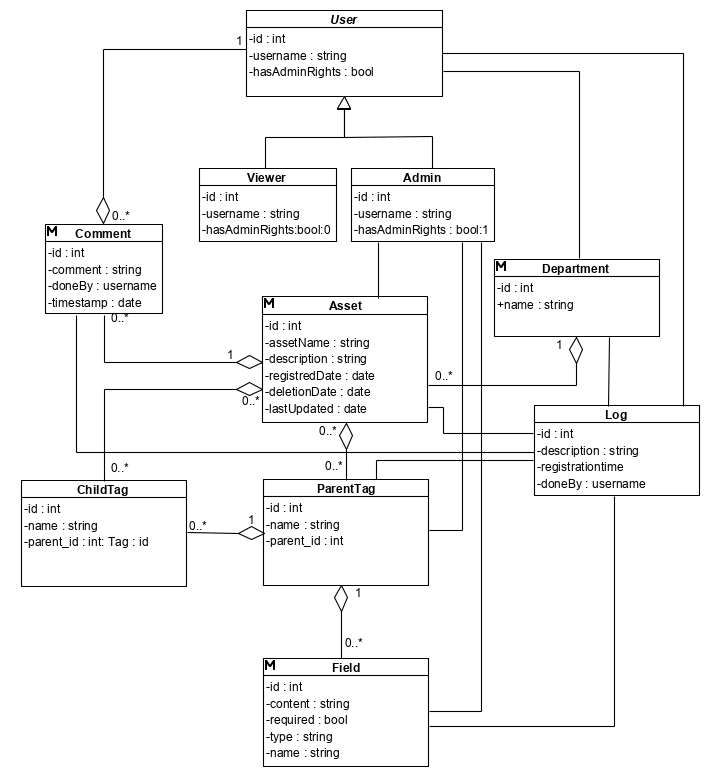
\includegraphics[width=1\textwidth]{figures/ClassDiagrams/ClassDiagramV6.PNG}
    \caption{Implementation class diagram (The bold M on some of the classes, is just a program specific thing, and can be ignored.)}
    \label{fig:CompleteClassDiagram}
\end{figure}

The class diagram in \autoref{fig:CompleteClassDiagram} shows the classes within the implemented system, as well as their internal relations. In this diagram some classes have been excluded, as these would cause unnecessary clutter in the diagram. The classes excluded from the diagram are \textit{Repositories} and \textit{ViewModels}. The excluded classes are components from the technical platform \autoref{sc:tech_intro}, as these control the data access layer and UI, and therefor do not represent key components in the logic of the system. 
\par
As seen on \autoref{fig:CompleteClassDiagram} the \textit{Log} class has an association to most of the classes within the system, as Aalborg Zoo requested that all changes should be logged. 


%%%%%%%%%%%%%%%%%%%%%%%%%%%%%%%%%%%%%%%%%%%%%%%%%%%%%%%%%%%%%%%
% Conclusion
%%%%%%%%%%%%%%%%%%%%%%%%%%%%%%%%%%%%%%%%%%%%%%%%%%%%%%%%%%%%%%%
\chapter{Conclusion}\label{ch:conclusion}




%%% End of document
\printbibliography[heading=bibintoc]
\label{bib:mybiblio}
\appendix
%\chapter{Appendix A name}\label{ch:appAlabel}
Here is the first appendix

\end{document}
